% Формат А4, 14pt (ГОСТ Р 7.0.11-2011, 5.3.6)
\documentclass[a4paper,14pt]{extreport}

%%%%%%%%%%%%%%%%%%%%%%%%%%%%%%%%%%%%%%%%%%%%%%%%%%%%%%
%%%% Файл упрощённых настроек шаблона диссертации %%%%
%%%%%%%%%%%%%%%%%%%%%%%%%%%%%%%%%%%%%%%%%%%%%%%%%%%%%%

%%%        Подключение пакетов                 %%%
\usepackage{ifthen}                 % добавляет ifthenelse
%%% Инициализирование переменных, не трогать!  %%%
\newcounter{intvl}
\newcounter{otstup}
\newcounter{contnum}
\newcounter{pgnum}
\newcounter{bibliosel}
\newcounter{chapstyle}
\newcounter{headingdelim}
\newcounter{headingalign}
\newcounter{headingsize}
\newcounter{tabcap}
\newcounter{tablaba}
\newcounter{tabtita}
%%%%%%%%%%%%%%%%%%%%%%%%%%%%%%%%%%%%%%%%%%%%%%%%%%

%%% Область упрощённого управления оформлением %%%

%% Интервал между заголовками и между заголовком и текстом
% Заголовки отделяют от текста сверху и снизу тремя интервалами (ГОСТ Р 7.0.11-2011, 5.3.5)
\setcounter{intvl}{3}               % Коэффициент кратности к размеру шрифта

%% Отступы у заголовков в тексте
\setcounter{otstup}{0}              % 0 --- без отступа; 1 --- абзацный отступ

%% Нумерация формул, таблиц и рисунков
\setcounter{contnum}{0}             % 0 --- пораздельно (во введении подряд, без номера раздела); 1 --- сквозная нумерация по всей диссертации

%% Оглавление
\setcounter{pgnum}{1}               % 0 --- номера страниц никак не обозначены; 1 --- Стр. над номерами страниц (дважды компилировать после изменения)

%% Библиография
\setcounter{bibliosel}{0}           % 0 --- встроенная реализация с загрузкой файла через движок bibtex8; 1 --- реализация пакетом biblatex через движок biber

%% Текст и форматирование заголовков
\setcounter{chapstyle}{1}           % 0 --- разделы только под номером; 1 --- разделы с названием "Глава" перед номером
\setcounter{headingdelim}{1}        % 0 --- номер отделен пропуском в 1em или \quad; 1 --- номера разделов и приложений отделены точкой с пробелом, подразделы пропуском без точки; 2 --- номера разделов, подразделов и приложений отделены точкой с пробелом.

%% Выравнивание заголовков в тексте
\setcounter{headingalign}{0}        % 0 --- по центру; 1 --- по левому краю

%% Размеры заголовков в тексте
\setcounter{headingsize}{0}         % 0 --- по ГОСТ, все всегда 14 пт; 1 --- пропорционально изменяющийся размер в зависимости от базового шрифта

%% Подпись таблиц
\setcounter{tabcap}{0}              % 0 --- по ГОСТ, номер таблицы и название разделены тире, выровнены по левому краю, при необходимости на нескольких строках; 1 --- подпись таблицы не по ГОСТ, на двух и более строках, дальнейшие настройки: 
%Выравнивание первой строки, с подписью и номером
\setcounter{tablaba}{2}             % 0 --- по левому краю; 1 --- по центру; 2 --- по правому краю
%Выравнивание строк с самим названием таблицы
\setcounter{tabtita}{1}             % 0 --- по левому краю; 1 --- по центру; 2 --- по правому краю               % Упрощённые настройки шаблона 

%%% Проверка используемого TeX-движка %%%
\usepackage{iftex}
\newif\ifxetexorluatex   % определяем новый условный оператор (http://tex.stackexchange.com/a/47579/79756)
\ifXeTeX
    \xetexorluatextrue
\else
    \ifLuaTeX
        \xetexorluatextrue
    \else
        \xetexorluatexfalse
    \fi
\fi

%%% Поля и разметка страницы %%%
\usepackage{pdflscape}                              % Для включения альбомных страниц
\usepackage{geometry}                               % Для последующего задания полей

%%% Математические пакеты %%%
\usepackage{amsthm,amsfonts,amsmath,amssymb,amscd}  % Математические дополнения от AMS
\usepackage{mathtools}                              % Добавляет окружение multlined

%%%% Установки для размера шрифта 14 pt %%%%
%% Формирование переменных и констант для сравнения (один раз для всех подключаемых файлов)%%
%% должно располагаться до вызова пакета fontspec или polyglossia, потому что они сбивают его работу
\newlength{\curtextsize}
\newlength{\bigtextsize}
\setlength{\bigtextsize}{13.9pt}

\makeatletter
%\show\f@size                                       % неплохо для отслеживания, но вызывает стопорение процесса, если документ компилируется без команды  -interaction=nonstopmode 
\setlength{\curtextsize}{\f@size pt}
\makeatother

%%% Кодировки и шрифты %%%
\ifxetexorluatex
    \usepackage{polyglossia}                        % Поддержка многоязычности (fontspec подгружается автоматически)
\else
    \RequirePDFTeX                                  % tests for PDFTEX use and throws an error if a different engine is being used
    \usepackage{cmap}                               % Улучшенный поиск русских слов в полученном pdf-файле
    \usepackage[T2A]{fontenc}                       % Поддержка русских букв
    \usepackage[utf8]{inputenc}                     % Кодировка utf8
    \usepackage[english, russian]{babel}            % Языки: русский, английский
    \IfFileExists{pscyr.sty}{\usepackage{pscyr}}{}  % Красивые русские шрифты
\fi

%%% Оформление абзацев %%%
\usepackage{indentfirst}                            % Красная строка

%%% Цвета %%%
\usepackage[dvipsnames,usenames]{color}
\usepackage{colortbl}

%%% Таблицы %%%
\usepackage{longtable}                              % Длинные таблицы
\usepackage{multirow,makecell,array}                % Улучшенное форматирование таблиц
\usepackage{booktabs}                               % Возможность оформления таблиц в классическом книжном стиле (при правильном использовании не противоречит ГОСТ)

%%% Общее форматирование
\usepackage{soulutf8}                               % Поддержка переносоустойчивых подчёркиваний и зачёркиваний
\usepackage{icomma}                                 % Запятая в десятичных дробях


%%% Гиперссылки %%%
\usepackage{hyperref}

%%% Изображения %%%
\usepackage{graphicx}                               % Подключаем пакет работы с графикой

%%% Списки %%%
\usepackage{enumitem}

%%% Подписи %%%
\usepackage{caption}                                % Для управления подписями (рисунков и таблиц) % Может управлять номерами рисунков и таблиц с caption %Иногда может управлять заголовками в списках рисунков и таблиц
\usepackage{subcaption}                             % Работа с подрисунками и подобным

%%% Интервалы %%%
\usepackage[onehalfspacing]{setspace}               % Опция запуска пакета правит не только интервалы в обычном тексте, но и формульные

%%% Счётчики %%%
\usepackage[figure,table]{totalcount}               % Счётчик рисунков и таблиц
\usepackage{totcount}                               % Пакет создания счётчиков на основе последнего номера подсчитываемого элемента (может требовать дважды компилировать документ)
\usepackage{totpages}                               % Счётчик страниц, совместимый с hyperref (ссылается на номер последней страницы). Желательно ставить последним пакетом в преамбуле

  % Пакеты общие для диссертации и автореферата
%%% Колонтитулы %%%
\usepackage{fancyhdr}

%%% Прикладные пакеты %%% 
\usepackage{calc}               % Пакет для расчётов параметров, например длины
%\usepackage{etoolbox}          % ради функции patchcmd для управления списком литературы

\usepackage {interfaces-base}   % Набор базовых интерфейсов к некоторым пакетам, конкретные реализации загружаются в стиле

%%% Заголовки %%%
\usepackage{titlesec}           % Пакет настройки шрифтов заголовков в тексте

%%% Оглавление %%%
\usepackage{tocloft}

%%% Счётчики %%%
\usepackage{chngcntr}           % оперативная перенастройка счётчиков         % Пакеты для диссертации
\usepackage{tabularx,tabulary}  %таблицы с автоматически подбирающейся шириной столбцов

% Листинги с исходным кодом программ
\usepackage{fancyvrb}
\usepackage{listings}

% Плавающие окружения. во многом лучше пакета float
\usepackage{floatrow}
        % Пакеты для специфических пользовательских задач
%%% Переопределение именований, чтобы можно было и в преамбуле использовать %%%
\renewcommand{\chaptername}{Глава}
\renewcommand{\appendixname}{Приложение} % (ГОСТ Р 7.0.11-2011, 5.7)
       % Переопределение именований, чтобы можно было и в преамбуле использовать
%%% Макет страницы %%%
% Выставляем значения полей (ГОСТ 7.0.11-2011, 5.3.7)
\geometry{a4paper,top=2cm,bottom=2cm,left=2.5cm,right=1cm}

%%% Кодировки и шрифты %%%
\ifxetexorluatex
    \setmainlanguage[babelshorthands=true]{russian}  % Язык по-умолчанию русский с поддержкой приятных команд пакета babel
    \setotherlanguage{english}                       % Дополнительный язык = английский (в американской вариации по-умолчанию)
    \ifXeTeX
        \defaultfontfeatures{Ligatures=TeX,Mapping=tex-text}
    \else
        \defaultfontfeatures{Ligatures=TeX}
    \fi
    \setmainfont{Times New Roman}
    \newfontfamily\cyrillicfont{Times New Roman}
    \setsansfont{Arial}
    \newfontfamily\cyrillicfontsf{Arial}
    \setmonofont{Courier New}
    \newfontfamily\cyrillicfonttt{Courier New}
\else
    \IfFileExists{pscyr.sty}{\renewcommand{\rmdefault}{ftm}}{}
\fi

%%% Интервалы %%%
%linespread-реализация ближе к реализации полуторного интервала в ворде.
%setspace реализация заточена под шрифты 10, 11, 12pt, под остальные кегли хуже, но всё же ближе к типографской классике. 
%\linespread{1.3}                    % Полуторный интервал (ГОСТ Р 7.0.11-2011, 5.3.6)

%%% Выравнивание и переносы %%%
\sloppy                             % Избавляемся от переполнений
\clubpenalty=10000                  % Запрещаем разрыв страницы после первой строки абзаца
\widowpenalty=10000                 % Запрещаем разрыв страницы после последней строки абзаца

%%% Изображения %%%
\graphicspath{{../assets/}}         % Пути к изображениям

%%% Подписи %%%
\captionsetup{%
singlelinecheck=off,                % Многострочные подписи, например у таблиц
skip=2pt,                           % Вертикальная отбивка между подписью и содержимым рисунка или таблицы определяется ключом
justification=centering,            % Центрирование подписей, заданных командой \caption
}

%%% Рисунки %%%
\DeclareCaptionLabelSeparator*{emdash}{~--- }             % (ГОСТ 2.105, 4.3.1)
\captionsetup[figure]{labelsep=emdash,font=onehalfspacing,position=bottom}

%%% Таблицы %%%
\ifthenelse{\equal{\thetabcap}{0}}{%
    \newcommand{\tabcapalign}{\raggedright}  % по левому краю страницы или аналога parbox
}

\ifthenelse{\equal{\thetablaba}{0} \AND \equal{\thetabcap}{1}}{%
    \newcommand{\tabcapalign}{\raggedright}  % по левому краю страницы или аналога parbox
}

\ifthenelse{\equal{\thetablaba}{1} \AND \equal{\thetabcap}{1}}{%
    \newcommand{\tabcapalign}{\centering}    % по центру страницы или аналога parbox
}

\ifthenelse{\equal{\thetablaba}{2} \AND \equal{\thetabcap}{1}}{%
    \newcommand{\tabcapalign}{\raggedleft}   % по правому краю страницы или аналога parbox
}

\ifthenelse{\equal{\thetabtita}{0} \AND \equal{\thetabcap}{1}}{%
    \newcommand{\tabtitalign}{\raggedright}  % по левому краю страницы или аналога parbox
}

\ifthenelse{\equal{\thetabtita}{1} \AND \equal{\thetabcap}{1}}{%
    \newcommand{\tabtitalign}{\centering}    % по центру страницы или аналога parbox
}

\ifthenelse{\equal{\thetabtita}{2} \AND \equal{\thetabcap}{1}}{%
    \newcommand{\tabtitalign}{\raggedleft}   % по правому краю страницы или аналога parbox
}

\ifthenelse{\equal{\thetabcap}{0}}{%
    \DeclareCaptionFormat{tablecaption}{\tabcapalign #1#2#3}
    \DeclareCaptionFormat{tablenocaption}{\tabcapalign #1#2}    % Наименование таблицы отсутствует
    \captionsetup[table]{labelsep=emdash}                       % тире как разделитель идентификатора с номером от наименования
}{%
    \DeclareCaptionFormat{tablecaption}{\tabcapalign #1#2\par%  % Идентификатор таблицы на отдельной строке
        \tabtitalign{#3}}                                       % Наименование таблицы строкой ниже
    \DeclareCaptionFormat{tablenocaption}{\tabcapalign #1#2}    % Наименование таблицы отсутствует
    \captionsetup[table]{labelsep=space}                        % пробельный разделитель идентификатора с номером от наименования
}
\captionsetup[table]{format=tablecaption,singlelinecheck=off,font=onehalfspacing,position=top,skip=0pt}  % многострочные наименования и прочее
\DeclareCaptionLabelFormat{continued}{Продолжение таблицы~#2}

%%% Подписи подрисунков %%%
\renewcommand{\thesubfigure}{\asbuk{subfigure}}           % Буквенные номера подрисунков
\captionsetup[subfigure]{font={normalsize},               % Шрифт подписи названий подрисунков (не отличается от основного)
    labelformat=brace,                                    % Формат обозначения подрисунка
    justification=centering,                              % Выключка подписей (форматирование), один из вариантов            
}
%\DeclareCaptionFont{font12pt}{\fontsize{12pt}{13pt}\selectfont} % объявляем шрифт 12pt для использования в подписях, тут же надо интерлиньяж объявлять, если не наследуется
%\captionsetup[subfigure]{font={font12pt}}                 % Шрифт подписи названий подрисунков (всегда 12pt)

%%% Цвета гиперссылок %%%
\definecolor{linkcolor}{rgb}{0.9,0,0}
\definecolor{citecolor}{rgb}{0,0.6,0}
\definecolor{urlcolor}{rgb}{0,0,1}

%%% Настройки гиперссылок %%%
\hypersetup{
    linktocpage=true,           % ссылки с номера страницы в оглавлении, списке таблиц и списке рисунков
%    pdfpagelabels=false,        % set PDF page labels (true|false)
    plainpages=false,           % Forces page anchors to be named by the Arabic form  of the page number, rather than the formatted form
    colorlinks,                 % ссылки отображаются раскрашенным текстом, а не раскрашенным прямоугольником, вокруг текста
    linkcolor={linkcolor},      % цвет ссылок типа ref, eqref и подобных
    citecolor={citecolor},      % цвет ссылок-цитат
    urlcolor={urlcolor},        % цвет гиперссылок
}

\ifLuaTeX
    \hypersetup{
        unicode,                % Unicode encoded PDF strings
    }
\fi

%%% Шаблон %%%
\DeclareRobustCommand{\todo}{\textcolor{red}}       % решаем проблему превращения названия цвета в результате \MakeUppercase, http://tex.stackexchange.com/a/187930/79756 , \DeclareRobustCommand protects \todo from expanding inside \MakeUppercase
\setlength{\parindent}{2.5em}                       % Абзацный отступ. Должен быть одинаковым по всему тексту и равен пяти знакам (ГОСТ Р 7.0.11-2011, 5.3.7).

%%% Списки %%%
% Используем дефис для ненумерованных списков (ГОСТ 2.105-95, 4.1.7)
\renewcommand{\labelitemi}{\normalfont\bfseries{--}} 
\setlist{nosep,%                                    % Единый стиль для всех списков (пакет enumitem), без дополнительных интервалов.
    labelindent=\parindent,leftmargin=*%            % Каждый пункт, подпункт и перечисление записывают с абзацного отступа (ГОСТ 2.105-95, 4.1.8)
}
    % Стили общие для диссертации и автореферата
\LoadInterface {titlesec}                   % Подгружаем интерфейсы для дополнительных опций управления некоторыми пакетами

%%% Блок управления параметрами для выравнивания заголовков в тексте %%%
\newlength{\otstuplen}
\setlength{\otstuplen}{\theotstup\parindent}
\ifthenelse{\equal{\theheadingalign}{0}}{% выравнивание заголовков в тексте
    \newcommand{\hdngalign}{\filcenter}                % по центру
    \newcommand{\hdngaligni}{\hfill\hspace{\otstuplen}}% по центру
}{%
    \newcommand{\hdngalign}{\filright}                 % по левому краю
    \newcommand{\hdngaligni}{\hspace{\otstuplen}}      % по левому краю
} % В обоих случаях вроде бы без переноса, как и надо (ГОСТ Р 7.0.11-2011, 5.3.5)

%%% Оглавление %%%
\renewcommand{\cftchapdotsep}{\cftdotsep}                % отбивка точками до номера страницы начала главы/раздела
\renewcommand{\cfttoctitlefont}{\hdngaligni\fontsize{14pt}{16pt}\selectfont\bfseries}% вместе со следующей строкой
\renewcommand{\cftaftertoctitle}{\hfill}                 % устанавливает заголовок по центру
\setlength{\cftbeforetoctitleskip}{-1.4\curtextsize}     % Поскольку этот заголовок всегда является первым на странице, то перед ним отделять пустым тройным интервалом не следует. Независимо от основного шрифта, в этом случае зануление (почти) происходит при -1.4\curtextsize.
\setlength{\cftaftertoctitleskip}{\theintvl\curtextsize} % Если считаем Оглавление заголовком, то выставляем после него тройной интервал через наше определённое значение

%% Переносить слова в заголовке не допускается (ГОСТ Р 7.0.11-2011, 5.3.5). Заголовки в оглавлении должны точно повторять заголовки в тексте (ГОСТ Р 7.0.11-2011, 5.2.3). Прямого указания на запрет переносов в оглавлении нет, но по той же логике невнесения искажений в смысл, лучше в оглавлении не переносить:
\cftsetrmarg{2.55em plus1fil}                       %To have the (sectional) titles in the ToC, etc., typeset ragged right with no hyphenation
\renewcommand{\cftchappagefont}{\normalfont}        % нежирные номера страниц у глав в оглавлении
\renewcommand{\cftchapleader}{\cftdotfill{\cftchapdotsep}}% нежирные точки до номеров страниц у глав в оглавлении
%\renewcommand{\cftchapfont}{}                       % нежирные названия глав в оглавлении

\ifthenelse{\theheadingdelim > 0}{%
    \renewcommand\cftchapaftersnum{.\ }   % добавляет точку с пробелом после номера раздела в оглавлении
}{%
\renewcommand\cftchapaftersnum{\quad}     % добавляет \quad после номера раздела в оглавлении
}
\ifthenelse{\theheadingdelim > 1}{%
    \renewcommand\cftsecaftersnum{.\ }    % добавляет точку с пробелом после номера подраздела в оглавлении
    \renewcommand\cftsubsecaftersnum{.\ } % добавляет точку с пробелом после номера подподраздела в оглавлении
}{%
\renewcommand\cftsecaftersnum{\quad}      % добавляет \quad после номера подраздела в оглавлении
\renewcommand\cftsubsecaftersnum{\quad}   % добавляет \quad после номера подподраздела в оглавлении
}

\ifthenelse{\equal{\thepgnum}{1}}{%
    \addtocontents{toc}{~\hfill{Стр.}\par}% добавить Стр. над номерами страниц
}

%%% Оформление названий глав %%%
%% настройки заголовка списка рисунков
\renewcommand{\cftloftitlefont}{\hdngaligni\fontsize{14pt}{16pt}\selectfont\bfseries}% вместе со следующей строкой
\renewcommand{\cftafterloftitle}{\hfill}                                             % устанавливает заголовок по центру
\setlength{\cftbeforeloftitleskip}{-1.5\curtextsize}     % Поскольку этот заголовок всегда является первым на странице, то перед ним отделять пустым тройным интервалом не следует. Независимо от основного шрифта, в этом случае зануление (почти) происходит при -1.5\curtextsize.
\setlength{\cftafterloftitleskip}{\theintvl\curtextsize} % выставляем после него тройной интервал через наше определённое значение

%% настройки заголовка списка таблиц
\renewcommand{\cftlottitlefont}{\hdngaligni\fontsize{14pt}{16pt}\selectfont\bfseries}% вместе со следующей строкой
\renewcommand{\cftafterlottitle}{\hfill}                                             % устанавливает заголовок по центру
\setlength{\cftbeforelottitleskip}{-1.5\curtextsize}     % Поскольку этот заголовок всегда является первым на странице, то перед ним отделять пустым тройным интервалом не следует. Независимо от основного шрифта, в этом случае зануление (почти) происходит при -1.5\curtextsize.
\setlength{\cftafterlottitleskip}{\theintvl\curtextsize} % выставляем после него тройной интервал через наше определённое значение

\ifnum\curtextsize>\bigtextsize     % Проверяем условие использования базового шрифта 14 pt
\setlength{\headheight}{17pt}       % Исправляем высоту заголовка
\else
\setlength{\headheight}{15pt}       % Исправляем высоту заголовка
\fi

%%% Колонтитулы %%%
% Порядковый номер страницы печатают на середине верхнего поля страницы (ГОСТ Р 7.0.11-2011, 5.3.8)
\makeatletter
\let\ps@plain\ps@fancy              % Подчиняем первые страницы каждой главы общим правилам
\makeatother
\pagestyle{fancy}                   % Меняем стиль оформления страниц
\fancyhf{}                          % Очищаем текущие значения
\fancyhead[C]{\thepage}             % Печатаем номер страницы на середине верхнего поля
\renewcommand{\headrulewidth}{0pt}  % Убираем разделительную линию

%%% Оформление заголовков глав, разделов, подразделов %%%
%% Работа должна быть выполнена ... размером шрифта 12-14 пунктов (ГОСТ Р 7.0.11-2011, 5.3.8). То есть не должно быть надписей шрифтом более 14. Так и поставим.
%% Эти установки будут давать одинаковый результат независимо от выбора базовым шрифтом 12 пт или 14 пт
\titleformat{\chapter}[block]                                % default display;  hang = with a hanging label. (Like the standard \section.); block = typesets the whole title in a block (a paragraph) without additional formatting. Useful in centered titles
        {\hdngalign\fontsize{14pt}{16pt}\selectfont\bfseries}% 
        %\fontsize{<size>}{<skip>} % второе число ставим 1.2*первое, чтобы адекватно отрабатывали команды по расчету полуторного интервала (домножая разные комбинации коэффициентов на этот)
        {\thechapter\cftchapaftersnum}                       % Заголовки в оглавлении должны точно повторять заголовки в тексте (ГОСТ Р 7.0.11-2011, 5.2.3).
        {0em}% отступ от номера до текста
        {}%

\titleformat{\section}[block]                                % default hang;  hang = with a hanging label. (Like the standard \section.); block = typesets the whole title in a block (a paragraph) without additional formatting. Useful in centered titles
        {\hdngalign\fontsize{14pt}{16pt}\selectfont\bfseries}% 
        %\fontsize{<size>}{<skip>} % второе число ставим 1.2*первое, чтобы адекватно отрабатывали команды по расчету полуторного интервала (домножая разные комбинации коэффициентов на этот)
        {\thesection\cftsecaftersnum}                        % Заголовки в оглавлении должны точно повторять заголовки в тексте (ГОСТ Р 7.0.11-2011, 5.2.3).
        {0em}% отступ от номера до текста
        {}%

\titleformat{\subsection}[block]                             % default hang;  hang = with a hanging label. (Like the standard \section.); block = typesets the whole title in a block (a paragraph) without additional formatting. Useful in centered titles
        {\hdngalign\fontsize{14pt}{16pt}\selectfont\bfseries}% 
        %\fontsize{<size>}{<skip>} % второе число ставим 1.2*первое, чтобы адекватно отрабатывали команды по расчету полуторного интервала (домножая разные комбинации коэффициентов на этот)
        {\thesubsection\cftsubsecaftersnum}                  % Заголовки в оглавлении должны точно повторять заголовки в тексте (ГОСТ Р 7.0.11-2011, 5.2.3).
        {0em}% отступ от номера до текста
        {}%

\ifthenelse{\equal{\thechapstyle}{1}}{%
    \sectionformat{\chapter}{% Параметры заголовков разделов в тексте
        label=\chaptername\ \thechapter\cftchapaftersnum,
        labelsep=0em,
    }
    %% Следующие две строки: будет вписано слово Глава перед каждым номером раздела в оглавлении   
    \renewcommand{\cftchappresnum}{\chaptername\ }
    \setlength{\cftchapnumwidth}{\widthof{\cftchapfont\cftchappresnum\thechapter\cftchapaftersnum}}
}%

%% Интервалы между заголовками
% На эти величины titlespacing множит через *
\beforetitleunit=\curtextsize% привязались к нашему размеру шрифта
\aftertitleunit=\curtextsize% привязались к нашему размеру шрифта

% Счётчик intvl и длина \otstup определены в файле setup
\titlespacing{\chapter}{\theotstup\parindent}{-1.7em}{*\theintvl}       % Заголовки отделяют от текста сверху и снизу тремя интервалами (ГОСТ Р 7.0.11-2011, 5.3.5). Поскольку название главы всегда является первым на странице, то перед ним отделять пустым тройным интервалом не следует. Независимо от основного шрифта, в этом случае зануление происходит при -1.7em.
\titlespacing{\section}{\theotstup\parindent}{*\theintvl}{*\theintvl}
\titlespacing{\subsection}{\theotstup\parindent}{*\theintvl}{*\theintvl}
\titlespacing{\subsubsection}{\theotstup\parindent}{*\theintvl}{*\theintvl}

%%% Блок дополнительного управления размерами заголовков
\ifthenelse{\equal{\theheadingsize}{1}}{% Пропорциональные заголовки и базовый шрифт 14 пт
    \renewcommand{\cfttoctitlefont}{\hdngaligni\Large\bfseries} % Исправляем размер заголовка оглавления
    \setlength{\cftbeforetoctitleskip}{-1.2\curtextsize}        % Исправляем вертикальный отступ перед заголовком оглавления
    \renewcommand{\cftloftitlefont}{\hdngaligni\Large\bfseries} % Исправляем размер заголовка списка рисунков
    \setlength{\cftbeforeloftitleskip}{-1.4\curtextsize}        % Исправляем вертикальный отступ перед заголовком списка рисунков
    \renewcommand{\cftlottitlefont}{\hdngaligni\Large\bfseries} % Исправляем размер заголовка списка таблиц 
    \setlength{\cftbeforelottitleskip}{-1.4\curtextsize}        % Исправляем вертикальный отступ перед заголовком списка таблиц
    \sectionformat{\chapter}{% Параметры заголовков разделов в тексте
        format=\hdngalign\Large\bfseries, % Исправляем размер заголовка
        top-=0.4em,                       % Исправляем вертикальный отступ перед заголовком
    }
    \sectionformat{\section}{% Параметры заголовков подразделов в тексте
        format=\hdngalign\large\bfseries, % Исправляем размер заголовка
    }
}

\ifthenelse{\equal{\theheadingsize}{1}\AND \curtextsize < \bigtextsize}{% Пропорциональные заголовки и базовый шрифт 14 пт
    \sectionformat{\chapter}{% Параметры заголовков разделов в тексте
        top-=0.2em, % Исправляем вертикальный отступ перед заголовком
    }
}

%%% Счётчики %%%

%% Упрощённые настройки шаблона диссертации: нумерация формул, таблиц, рисунков
\ifthenelse{\equal{\thecontnum}{1}}{%
    \counterwithout{equation}{chapter} % Убираем связанность номера формулы с номером главы/раздела
    \counterwithout{figure}{chapter}   % Убираем связанность номера рисунка с номером главы/раздела
    \counterwithout{table}{chapter}    % Убираем связанность номера таблицы с номером главы/раздела
}

%%http://www.linux.org.ru/forum/general/6993203#comment-6994589 (используется totcount)
\makeatletter
\def\formbytotal#1#2#3#4#5{%
    \newcount\@c
    \@c\totvalue{#1}\relax
    \newcount\@last
    \newcount\@pnul
    \@last\@c\relax
    \divide\@last 10
    \@pnul\@last\relax
    \divide\@pnul 10
    \multiply\@pnul-10
    \advance\@pnul\@last
    \multiply\@last-10
    \advance\@last\@c
    \total{#1}~#2%
    \ifnum\@pnul=1#5\else%
    \ifcase\@last#5\or#3\or#4\or#4\or#4\else#5\fi
    \fi
}
\makeatother
           % Стили для диссертации
% для вертикального центрирования ячеек в tabulary
\def\zz{\ifx\[$\else\aftergroup\zzz\fi}
\def\zzz{\setbox0\lastbox
\dimen0\dimexpr\extrarowheight + \ht0-\dp0\relax
\setbox0\hbox{\raise-.5\dimen0\box0}%
\ht0=\dimexpr\ht0+\extrarowheight\relax
\dp0=\dimexpr\dp0+\extrarowheight\relax 
\box0
}



\lstdefinelanguage{Renhanced}%
{keywords={abbreviate,abline,abs,acos,acosh,action,add1,add,%
        aggregate,alias,Alias,alist,all,anova,any,aov,aperm,append,apply,%
        approx,approxfun,apropos,Arg,args,array,arrows,as,asin,asinh,%
        atan,atan2,atanh,attach,attr,attributes,autoload,autoloader,ave,%
        axis,backsolve,barplot,basename,besselI,besselJ,besselK,besselY,%
        beta,binomial,body,box,boxplot,break,browser,bug,builtins,bxp,by,%
        c,C,call,Call,case,cat,category,cbind,ceiling,character,char,%
        charmatch,check,chol,chol2inv,choose,chull,class,close,cm,codes,%
        coef,coefficients,co,col,colnames,colors,colours,commandArgs,%
        comment,complete,complex,conflicts,Conj,contents,contour,%
        contrasts,contr,control,helmert,contrib,convolve,cooks,coords,%
        distance,coplot,cor,cos,cosh,count,fields,cov,covratio,wt,CRAN,%
        create,crossprod,cummax,cummin,cumprod,cumsum,curve,cut,cycle,D,%
        data,dataentry,date,dbeta,dbinom,dcauchy,dchisq,de,debug,%
        debugger,Defunct,default,delay,delete,deltat,demo,de,density,%
        deparse,dependencies,Deprecated,deriv,description,detach,%
        dev2bitmap,dev,cur,deviance,off,prev,,dexp,df,dfbetas,dffits,%
        dgamma,dgeom,dget,dhyper,diag,diff,digamma,dim,dimnames,dir,%
        dirname,dlnorm,dlogis,dnbinom,dnchisq,dnorm,do,dotplot,double,%
        download,dpois,dput,drop,drop1,dsignrank,dt,dummy,dump,dunif,%
        duplicated,dweibull,dwilcox,dyn,edit,eff,effects,eigen,else,%
        emacs,end,environment,env,erase,eval,equal,evalq,example,exists,%
        exit,exp,expand,expression,External,extract,extractAIC,factor,%
        fail,family,fft,file,filled,find,fitted,fivenum,fix,floor,for,%
        For,formals,format,formatC,formula,Fortran,forwardsolve,frame,%
        frequency,ftable,ftable2table,function,gamma,Gamma,gammaCody,%
        gaussian,gc,gcinfo,gctorture,get,getenv,geterrmessage,getOption,%
        getwd,gl,glm,globalenv,gnome,GNOME,graphics,gray,grep,grey,grid,%
        gsub,hasTsp,hat,heat,help,hist,home,hsv,httpclient,I,identify,if,%
        ifelse,Im,image,\%in\%,index,influence,measures,inherits,install,%
        installed,integer,interaction,interactive,Internal,intersect,%
        inverse,invisible,IQR,is,jitter,kappa,kronecker,labels,lapply,%
        layout,lbeta,lchoose,lcm,legend,length,levels,lgamma,library,%
        licence,license,lines,list,lm,load,local,locator,log,log10,log1p,%
        log2,logical,loglin,lower,lowess,ls,lsfit,lsf,ls,machine,Machine,%
        mad,mahalanobis,make,link,margin,match,Math,matlines,mat,matplot,%
        matpoints,matrix,max,mean,median,memory,menu,merge,methods,min,%
        missing,Mod,mode,model,response,mosaicplot,mtext,mvfft,na,nan,%
        names,omit,nargs,nchar,ncol,NCOL,new,next,NextMethod,nextn,%
        nlevels,nlm,noquote,NotYetImplemented,NotYetUsed,nrow,NROW,null,%
        numeric,\%o\%,objects,offset,old,on,Ops,optim,optimise,optimize,%
        options,or,order,ordered,outer,package,packages,page,pairlist,%
        pairs,palette,panel,par,parent,parse,paste,path,pbeta,pbinom,%
        pcauchy,pchisq,pentagamma,persp,pexp,pf,pgamma,pgeom,phyper,pico,%
        pictex,piechart,Platform,plnorm,plogis,plot,pmatch,pmax,pmin,%
        pnbinom,pnchisq,pnorm,points,poisson,poly,polygon,polyroot,pos,%
        postscript,power,ppoints,ppois,predict,preplot,pretty,Primitive,%
        print,prmatrix,proc,prod,profile,proj,prompt,prop,provide,%
        psignrank,ps,pt,ptukey,punif,pweibull,pwilcox,q,qbeta,qbinom,%
        qcauchy,qchisq,qexp,qf,qgamma,qgeom,qhyper,qlnorm,qlogis,qnbinom,%
        qnchisq,qnorm,qpois,qqline,qqnorm,qqplot,qr,Q,qty,qy,qsignrank,%
        qt,qtukey,quantile,quasi,quit,qunif,quote,qweibull,qwilcox,%
        rainbow,range,rank,rbeta,rbind,rbinom,rcauchy,rchisq,Re,read,csv,%
        csv2,fwf,readline,socket,real,Recall,rect,reformulate,regexpr,%
        relevel,remove,rep,repeat,replace,replications,report,require,%
        resid,residuals,restart,return,rev,rexp,rf,rgamma,rgb,rgeom,R,%
        rhyper,rle,rlnorm,rlogis,rm,rnbinom,RNGkind,rnorm,round,row,%
        rownames,rowsum,rpois,rsignrank,rstandard,rstudent,rt,rug,runif,%
        rweibull,rwilcox,sample,sapply,save,scale,scan,scan,screen,sd,se,%
        search,searchpaths,segments,seq,sequence,setdiff,setequal,set,%
        setwd,show,sign,signif,sin,single,sinh,sink,solve,sort,source,%
        spline,splinefun,split,sqrt,stars,start,stat,stem,step,stop,%
        storage,strstrheight,stripplot,strsplit,structure,strwidth,sub,%
        subset,substitute,substr,substring,sum,summary,sunflowerplot,svd,%
        sweep,switch,symbol,symbols,symnum,sys,status,system,t,table,%
        tabulate,tan,tanh,tapply,tempfile,terms,terrain,tetragamma,text,%
        time,title,topo,trace,traceback,transform,tri,trigamma,trunc,try,%
        ts,tsp,typeof,unclass,undebug,undoc,union,unique,uniroot,unix,%
        unlink,unlist,unname,untrace,update,upper,url,UseMethod,var,%
        variable,vector,Version,vi,warning,warnings,weighted,weights,%
        which,while,window,write,\%x\%,x11,X11,xedit,xemacs,xinch,xor,%
        xpdrows,xy,xyinch,yinch,zapsmall,zip},%
    otherkeywords={!,!=,~,$,*,\%,\&,\%/\%,\%*\%,\%\%,<-,<<-},%
    alsoother={._$},%
    sensitive,%
    morecomment=[l]\#,%
    morestring=[d]",%
    morestring=[d]'% 2001 Robert Denham
}%

%решаем проблему с кириллицей в комментариях (в pdflatex) https://tex.stackexchange.com/a/103712/79756
\lstset{extendedchars=true,literate={Ö}{{\"O}}1
    {Ä}{{\"A}}1
    {Ü}{{\"U}}1
    {ß}{{\ss}}1
    {ü}{{\"u}}1
    {ä}{{\"a}}1
    {ö}{{\"o}}1
    {~}{{\textasciitilde}}1
    {а}{{\selectfont\char224}}1
    {б}{{\selectfont\char225}}1
    {в}{{\selectfont\char226}}1
    {г}{{\selectfont\char227}}1
    {д}{{\selectfont\char228}}1
    {е}{{\selectfont\char229}}1
    {ё}{{\"e}}1
    {ж}{{\selectfont\char230}}1
    {з}{{\selectfont\char231}}1
    {и}{{\selectfont\char232}}1
    {й}{{\selectfont\char233}}1
    {к}{{\selectfont\char234}}1
    {л}{{\selectfont\char235}}1
    {м}{{\selectfont\char236}}1
    {н}{{\selectfont\char237}}1
    {о}{{\selectfont\char238}}1
    {п}{{\selectfont\char239}}1
    {р}{{\selectfont\char240}}1
    {с}{{\selectfont\char241}}1
    {т}{{\selectfont\char242}}1
    {у}{{\selectfont\char243}}1
    {ф}{{\selectfont\char244}}1
    {х}{{\selectfont\char245}}1
    {ц}{{\selectfont\char246}}1
    {ч}{{\selectfont\char247}}1
    {ш}{{\selectfont\char248}}1
    {щ}{{\selectfont\char249}}1
    {ъ}{{\selectfont\char250}}1
    {ы}{{\selectfont\char251}}1
    {ь}{{\selectfont\char252}}1
    {э}{{\selectfont\char253}}1
    {ю}{{\selectfont\char254}}1
    {я}{{\selectfont\char255}}1
    {А}{{\selectfont\char192}}1
    {Б}{{\selectfont\char193}}1
    {В}{{\selectfont\char194}}1
    {Г}{{\selectfont\char195}}1
    {Д}{{\selectfont\char196}}1
    {Е}{{\selectfont\char197}}1
    {Ё}{{\"E}}1
    {Ж}{{\selectfont\char198}}1
    {З}{{\selectfont\char199}}1
    {И}{{\selectfont\char200}}1
    {Й}{{\selectfont\char201}}1
    {К}{{\selectfont\char202}}1
    {Л}{{\selectfont\char203}}1
    {М}{{\selectfont\char204}}1
    {Н}{{\selectfont\char205}}1
    {О}{{\selectfont\char206}}1
    {П}{{\selectfont\char207}}1
    {Р}{{\selectfont\char208}}1
    {С}{{\selectfont\char209}}1
    {Т}{{\selectfont\char210}}1
    {У}{{\selectfont\char211}}1
    {Ф}{{\selectfont\char212}}1
    {Х}{{\selectfont\char213}}1
    {Ц}{{\selectfont\char214}}1
    {Ч}{{\selectfont\char215}}1
    {Ш}{{\selectfont\char216}}1
    {Щ}{{\selectfont\char217}}1
    {Ъ}{{\selectfont\char218}}1
    {Ы}{{\selectfont\char219}}1
    {Ь}{{\selectfont\char220}}1
    {Э}{{\selectfont\char221}}1
    {Ю}{{\selectfont\char222}}1
    {Я}{{\selectfont\char223}}1
    {і}{{\selectfont\char105}}1
    {ї}{{\selectfont\char168}}1
    {є}{{\selectfont\char185}}1
    {ґ}{{\selectfont\char160}}1
    {І}{{\selectfont\char73}}1
    {Ї}{{\selectfont\char136}}1
    {Є}{{\selectfont\char153}}1
    {Ґ}{{\selectfont\char128}}1
}

% Ширина текста минус ширина надписи 999
\newlength{\twless}
\newlength{\lmarg}
\setlength{\lmarg}{\widthof{999}}   % ширина надписи 999
\setlength{\twless}{\textwidth-\lmarg}


\lstset{ %
%    language=R,                     %  Язык указать здесь, если во всех листингах преимущественно один язык, в результате часть настроек может пойти только для этого языка
    numbers=left,                   % where to put the line-numbers
    numberstyle=\fontsize{12pt}{14pt}\selectfont\color{Gray},  % the style that is used for the line-numbers
    firstnumber=2,                  % в этой и следующей строках задаётся поведение нумерации 5, 10, 15...
    stepnumber=5,                   % the step between two line-numbers. If it's 1, each line will be numbered
    numbersep=5pt,                  % how far the line-numbers are from the code
    backgroundcolor=\color{white},  % choose the background color. You must add \usepackage{color}
    showspaces=false,               % show spaces adding particular underscores
    showstringspaces=false,         % underline spaces within strings
    showtabs=false,                 % show tabs within strings adding particular underscores
    frame=leftline,                 % adds a frame of different types around the code
    rulecolor=\color{black},        % if not set, the frame-color may be changed on line-breaks within not-black text (e.g. commens (green here))
    tabsize=2,                      % sets default tabsize to 2 spaces
    captionpos=t,                   % sets the caption-position to top
    breaklines=true,                % sets automatic line breaking
    breakatwhitespace=false,        % sets if automatic breaks should only happen at whitespace
%    title=\lstname,                 % show the filename of files included with \lstinputlisting;
    % also try caption instead of title
    basicstyle=\fontsize{12pt}{14pt}\selectfont\ttfamily,% the size of the fonts that are used for the code
%    keywordstyle=\color{blue},      % keyword style
    commentstyle=\color{ForestGreen}\emph,% comment style
    stringstyle=\color{Mahogany},   % string literal style
    escapeinside={\%*}{*)},         % if you want to add a comment within your code
    morekeywords={*,...},           % if you want to add more keywords to the set
    inputencoding=utf8,             % кодировка кода
    xleftmargin={\lmarg},           % Чтобы весь код и полоска с номерами строк была смещена влево, так чтобы цифры не вылезали за пределы текста слева
} 

%http://tex.stackexchange.com/questions/26872/smaller-frame-with-listings
% Окружение, чтобы листинг был компактнее обведен рамкой, если она задается, а не на всю ширину текста
\makeatletter
\newenvironment{SmallListing}[1][]
{\lstset{#1}\VerbatimEnvironment\begin{VerbatimOut}{VerbEnv.tmp}}
{\end{VerbatimOut}\settowidth\@tempdima{%
        \lstinputlisting{VerbEnv.tmp}}
    \minipage{\@tempdima}\lstinputlisting{VerbEnv.tmp}\endminipage}    
\makeatother


\DefineVerbatimEnvironment% с шрифтом 12 пт
{Verb}{Verbatim}
{fontsize=\fontsize{12pt}{14pt}\selectfont}

\RawFloats[figure,table]            % Отмена установок пакета floatrow для всех флотов (плавающих окружений) выбранных типов или подтипов. А то будто мы зря задавали настройки подписей рисунков и таблиц. 

\DeclareNewFloatType{ListingEnv}{
    placement=htb,
    within=chapter,
    fileext=lol,
    name=Листинг,
}

\captionsetup[ListingEnv]{
    format=tablecaption,
    labelsep=space,                 % Точка после номера листинга задается значением period
    singlelinecheck=off,
    font=onehalfspacing,
    position=top,
}


\floatsetup[ListingEnv]{
    style=plaintop,
    captionskip=4pt,
}

\captionsetup[lstlisting]{
    format=tablecaption,
    labelsep=space,                 % Точка после номера листинга задается значением period
    singlelinecheck=off,
    font=onehalfspacing,
    position=top,
}

\renewcommand{\lstlistingname}{Листинг}

%Общие счётчики окружений листингов
%http://tex.stackexchange.com/questions/145546/how-to-make-figure-and-listing-share-their-counter
% Если смешивать плавающие и не плавающие окружения, то могут быть проблемы с нумерацией
\makeatletter
\AtBeginDocument{%
    \let\c@ListingEnv\c@lstlisting
    \let\theListingEnv\thelstlisting
    \let\ftype@lstlisting\ftype@ListingEnv % give the floats the same precedence
}
\makeatother

% значок С++ — используйте команду \cpp
\newcommand{\cpp}{%
    C\nolinebreak\hspace{-.05em}%
    \raisebox{.2ex}{+}\nolinebreak\hspace{-.10em}%
    \raisebox{.2ex}{+}%
}

          % Стили для специфических пользовательских задач
%%% Библиография. Общие настройки для двух способов её подключения %%%


%%% Выбор реализации %%%
\ifthenelse{\equal{\thebibliosel}{0}}{%
    %%% Реализация библиографии встроенными средствами посредством движка bibtex8 %%%

%%% Пакеты %%%
\usepackage{cite}                                   % Красивые ссылки на литературу


%%% Стили %%%
\bibliographystyle{../BibTeX-Styles/utf8gost71u}    % Оформляем библиографию по ГОСТ 7.1 (ГОСТ Р 7.0.11-2011, 5.6.7)

\makeatletter
\renewcommand{\@biblabel}[1]{#1.}   % Заменяем библиографию с квадратных скобок на точку
\makeatother
%% Управление отступами между записями
%% требует etoolbox 
%% http://tex.stackexchange.com/a/105642
%\patchcmd\thebibliography
% {\labelsep}
% {\labelsep\itemsep=5pt\parsep=0pt\relax}
% {}
% {\typeout{Couldn't patch the command}}

%%% Цитирование %%%
\renewcommand\citepunct{;\penalty\citepunctpenalty%
    \hskip.13emplus.1emminus.1em\relax}                % Разделение ; при перечислении ссылок (ГОСТ Р 7.0.5-2008)


%%% Создание команд для вывода списка литературы %%%
\newcommand*{\insertbibliofull}{
\bibliography{../biblio/othercites,../biblio/authorpapersVAK,../biblio/authorpapers,../biblio/authorconferences}         % Подключаем BibTeX-базы % После запятых не должно быть лишних пробелов — он "думает", что это тоже имя пути
}

\newcommand*{\insertbiblioauthor}{
\bibliography{../biblio/authorpapersVAK,../biblio/authorpapers,../biblio/authorconferences}         % Подключаем BibTeX-базы % После запятых не должно быть лишних пробелов — он "думает", что это тоже имя пути
}

\newcommand*{\insertbiblioother}{
\bibliography{../biblio/othercites}         % Подключаем BibTeX-базы
}

\newcommand*{\insertbiblioscopus}{
\bibliography{../biblio/biblio-scopus}         % Подключаем BibTeX-базы
}
\newcommand*{\insertbiblioall}{
\bibliography{../Dissertation/biblio}         % Подключаем BibTeX-базы
}


%% Счётчик использованных ссылок на литературу, обрабатывающий с учётом неоднократных ссылок
%% Требуется дважды компилировать, поскольку ему нужно считать актуальный внешний файл со списком литературы
\newtotcounter{citenum}
\def\oldcite{}
\let\oldcite=\bibcite
\def\bibcite{\stepcounter{citenum}\oldcite}
  % Встроенная реализация с загрузкой файла через движок bibtex8
}{
    %%% Реализация библиографии пакетами biblatex и biblatex-gost с использованием движка biber %%%

%\usepackage{csquotes} % biblatex рекомендует его подключать. Пакет для оформления сложных блоков цитирования.

%%% Загрузка пакета с основными настройками %%%
\usepackage[%
backend=biber,% движок
bibencoding=utf8,% кодировка bib файла
sorting=none,% настройка сортировки списка литературы
style=gost-numeric,% стиль цитирования и библиографии (по ГОСТ)
language=auto,% получение языка из babel/polyglossia
autolang=other,% многоязычная библиография
clearlang=true,% внутренний сброс поля language, если он совпадает с языком из babel/polyglossia
defernumbers=true,% нумерация проставляется после двух компиляций, зато позволяет выцеплять библиографию по ключевым словам и нумеровать не из большего списка
sortcites=true,% сортировать номера затекстовых ссылок при цитировании (если в квадратных скобках несколько ссылок, то отображаться будут отсортированно, а не абы как)
]{biblatex}



%http://tex.stackexchange.com/a/141831/79756
%There is a way to automatically map the language field to the langid field. The following lines in the preamble should be enough to do that.
%This command will copy the language field into the langid field and will then delete the contents of the language field. The language field will only be deleted if it was successfully copied into the langid field.
\DeclareSourcemap{ %модификация bib файла перед тем, как им займётся biblatex 
    \maps{
        \map{% перекидываем значения полей language в поля langid, которыми пользуется biblatex
            \step[fieldsource=language, fieldset=langid, origfieldval, final]
            \step[fieldset=language, null]
        }
        \map{% перекидываем значения полей numpages в поля pagetotal, которыми пользуется biblatex
            \step[fieldsource=numpages, fieldset=pagetotal, origfieldval, final]
            \step[fieldset=pagestotal, null]
        }
        \map{% если в поле medium написано "Электронный ресурс", то устанавливаем поле media. которым пользуется biblatex в значение eresource
            \step[fieldsource=medium,
            match=\regexp{Электронный\s+ресурс},
            final]
            \step[fieldset=media, fieldvalue=eresource]
        }
        \map[overwrite]{% стираем значения всех полей issn
            \step[fieldset=issn, null]
        }
        \map[overwrite]{% стираем значения всех полей abstract, поскольку ими не пользуемся, а там бывают "неприятные" латеху символы
            \step[fieldsource=abstract]
            \step[fieldset=abstract,null]
        }
        \map[overwrite]{ % переделка формата записи даты
            \step[fieldsource=urldate,
            match=\regexp{([0-9]{2})\.([0-9]{2})\.([0-9]{4})},
            replace={$3-$2-$1$4}, % $4 вставлен исключительно ради нормальной работы программ подсветки синтаксиса, которые некорректно обрабатывают $ в таких конструкциях
            final]
        }
        \map[overwrite]{ % добавляем ключевые слова, чтобы различать источники
            \perdatasource{../biblio/authorpapersVAK.bib}
            \perdatasource{../biblio/authorpapers.bib}
            \perdatasource{../biblio/authorconferences.bib}
            \step[fieldset=keywords, fieldvalue={biblioauthor}]
        }
        \map[overwrite]{ % добавляем ключевые слова, чтобы различать источники
            \perdatasource{../biblio/othercites.bib}
            \step[fieldset=keywords, fieldvalue={biblioother,bibliofull}]
        }
        \map[overwrite]{ % добавляем ключевые слова, чтобы различать источники
            \perdatasource{../biblio/othercites.bib}
            \step[fieldset=keywords, fieldvalue={biblioother,bibliofull}]
        }
    }
}

%\newbibmacro{string+doi}[1]{% новая макрокоманда на простановку ссылки на doi
%    \iffieldundef{doi}{#1}{\href{http://dx.doi.org/\thefield{doi}}{#1}}}
%
%\renewcommand*{\mkgostheading}[1]{\usebibmacro{string+doi}{#1}} % ссылка на doi с авторов. стоящих впереди записи
%\DeclareFieldFormat{title}{\usebibmacro{string+doi}{#1}} % ссылка на doi с названия работы
%\DeclareFieldFormat{journaltitle}{\usebibmacro{string+doi}{#1}} % ссылка на doi с названия журнала

%%% Подключение файлов bib %%%
\addbibresource{../biblio/othercites.bib}
\addbibresource{../biblio/authorpapersVAK.bib}
\addbibresource{../biblio/authorpapers.bib}
\addbibresource{../biblio/authorconferences.bib}


%% Счётчик использованных ссылок на литературу, обрабатывающий с учётом неоднократных ссылок
%http://tex.stackexchange.com/a/66851/79756
%\newcounter{citenum}
\newtotcounter{citenum}
\makeatletter
\defbibenvironment{counter}
  {\setcounter{citenum}{0}
  \renewcommand{\blx@driver}[1]{}
  }
  {} %\thecitenum сюда писать не надо
  {\stepcounter{citenum}}
\makeatother
\defbibheading{counter}{}

%%% Создание команд для вывода списка литературы %%%
\newcommand*{\insertbibliofull}{
\printbibliography[keyword=bibliofull]
\printbibliography[heading=counter,env=counter,keyword=bibliofull]
}

\newcommand*{\insertbiblioauthor}{
\printbibliography[keyword=biblioauthor]
\printbibliography[heading=counter,env=counter,keyword=biblioauthor]
}

\newcommand*{\insertbiblioother}{
\printbibliography[keyword=biblioother]
\printbibliography[heading=counter,env=counter,keyword=biblioother]
}


    % Реализация пакетом biblatex через движок biber
}
% Настройки библиографии из внешнего файла (там же выбор: встроенная или на основе biblatex)
%%% Основные сведения %%%

%%% Основные сведения %%%
\newcommand{\thesisAuthor}             % Диссертация, ФИО автора
{Тощев Александр Сергеевич}
\newcommand{\thesisUdk}                % Диссертация, УДК
{004.8}
\newcommand{\thesisTitle}              % Диссертация, название
{Интеллектуальная система повышения эффективности IT службы предприятия}

% Обобщение Модели Минского (обобщенная)
\newcommand{\thesisSpecialtyNumber}    % Диссертация, специальность, номер
{05.13.01}
\newcommand{\thesisSpecialtyTitle}     % Диссертация, специальность, название
{Системный анализ, управление и обработка информации (информационные технологии)}
\newcommand{\thesisDegree}             % Диссертация, научная степень
{Кандидат технических наук}
\newcommand{\thesisCity}               % Диссертация, город защиты
{Казань}
\newcommand{\thesisYear}               % Диссертация, год защиты
{2015}
\newcommand{\thesisOrganization}       % Диссертация, организация
{Казанский (Приволжский) Федеральный Университет\par}

\newcommand{\supervisorFio}            % Научный руководитель, ФИО
{Елизаров А.М.}
\newcommand{\supervisorRegalia}        % Научный руководитель, регалии
{доктор физико-математических наук, профессор}

\newcommand{\opponentOneFio}           % Оппонент 1, ФИО
{Соловьев Валерий Дмитриевич}
\newcommand{\opponentOneRegalia}       % Оппонент 1, регалии
{доктор физико-математических наук, профессор}
\newcommand{\opponentOneJobPlace}      % Оппонент 1, место работы
{Казанский (Приволжский) Федеральный Университет, Институт филологии и межкультурной коммуникации им. Льва Толстого}
\newcommand{\opponentOneJobPost}       % Оппонент 1, должность
{Ведущий научный сотрудник}
\newcommand{\opponentTwoFio}           % Оппонент 2, ФИО
{\todo{Оппонет2}}
\newcommand{\opponentTwoRegalia}       % Оппонент 2, регалии
{кандидат технических наук}
\newcommand{\opponentTwoJobPlace}      % Оппонент 2, место работы
{\todo{Оппонет2}}
\newcommand{\opponentTwoJobPost}       % Оппонент 2, должность
{\todo{Оппонет2}}

\newcommand{\leadingOrganizationTitle} % Ведущая организация, дополнительные строки
{Федеральное государственное бюджетное учреждение науки Институт проблем информатики Российской академии наук}

\newcommand{\defenseDate}              % Защита, дата
{\todo{DD mmmmmmmm YYYY~г.~в~XX часов}}
\newcommand{\defenseCouncilNumber}     % Защита, номер диссертационного совета
{\todo{NN}}
\newcommand{\defenseCouncilTitle}      % Защита, учреждение диссертационного совета
{\todo{Название учреждения}}
\newcommand{\defenseCouncilAddress}    % Защита, адрес учреждение диссертационного совета
{\todo{Адрес}}

\newcommand{\defenseSecretaryFio}      % Секретарь диссертационного совета, ФИО
{\todo{Фамилия Имя Отчество}}
\newcommand{\defenseSecretaryRegalia}  % Секретарь диссертационного совета, регалии
{\todo{д-р~физ.-мат. наук}}            % Для сокращений есть ГОСТы, например: ГОСТ Р 7.0.12-2011 + http://base.garant.ru/179724/#block_30000

\newcommand{\synopsisLibrary}          % Автореферат, название библиотеки
{\todo{Название библиотеки}}
\newcommand{\synopsisDate}             % Автореферат, дата рассылки
{\todo{DD mmmmmmmm YYYY года}}      % Основные сведения
\begin{document}
\lstset{language=Pascal} 
%%% Переопределение именований %%%
\renewcommand{\abstractname}{Аннотация}
\renewcommand{\alsoname}{см. также}
\renewcommand{\appendixname}{Приложение} % (ГОСТ Р 7.0.11-2011, 5.7)
\renewcommand{\bibname}{Список литературы} % (ГОСТ Р 7.0.11-2011, 4)
\renewcommand{\ccname}{исх.}
\renewcommand{\chaptername}{Глава}
\renewcommand{\contentsname}{Оглавление} % (ГОСТ Р 7.0.11-2011, 4)
\renewcommand{\enclname}{вкл.}
\renewcommand{\figurename}{Рисунок} % (ГОСТ Р 7.0.11-2011, 5.3.9)
\renewcommand{\headtoname}{вх.}
\renewcommand{\indexname}{Предметный указатель}
\renewcommand{\listfigurename}{Список рисунков}
\renewcommand{\listtablename}{Список таблиц}
\renewcommand{\pagename}{Стр.}
\renewcommand{\partname}{Часть}
\renewcommand{\refname}{Список литературы} % (ГОСТ Р 7.0.11-2011, 4)
\renewcommand{\seename}{см.}
\renewcommand{\tablename}{Таблица} % (ГОСТ Р 7.0.11-2011, 5.3.10)           % Переопределение именований
%test
% Структура диссертации (ГОСТ Р 7.0.11-2011, 4)
% Титульный лист (ГОСТ Р 7.0.11-2001, 5.1)
\thispagestyle{empty}

\begin{center}
\thesisOrganization \par
\par
\end{center}

\vspace{20mm}
\begin{flushright}
На правах рукописи

{\sl УДК \thesisUdk}
\end{flushright}

\vspace{30mm}
\begin{center}
{\large \thesisAuthor}
\end{center}

\vspace{5mm}
\begin{center}
{\bf \large \thesisTitle
\par}

\vspace{10mm}
{%\small
Специальность \thesisSpecialtyNumber~---

<<\thesisSpecialtyTitle>>
}

\vspace{10mm}
Диссертация на соискание учёной степени

\thesisDegree
\end{center}

\vspace{20mm}
\begin{flushright}
Научный руководитель:

\supervisorRegalia

\supervisorFio

\end{flushright}

\vspace{20mm}
\begin{center}
{\thesisCity~--- \thesisYear}
\end{center}

\newpage
           % Титульный лист
% Оглавление (ГОСТ Р 7.0.11-2011, 5.2)
\tableofcontents
\clearpage        % Оглавление
\chapter*{Введение}							% Заголовок
\addcontentsline{toc}{chapter}{Введение}	% Добавляем его в оглавление

В настоящее время все более популярным и распространенным становится процесс передачи функций поддержки информационной инфраструктуры (далее~--- ИТ-инфраструктуры) предприятия какой-либо внешней компании (см., например, \cite{StartToOutsource}). Это явление стало называться «ИТ-аутсорсинг» (от анг. ”out source”~--– вне источника). С развитием рынка компаниям становится невыгодно держать свой штат службы поддержки, и они отдают эти функции сторонней компании (см. \cite{OutsourceEff}). В некоторых случаях передаются все функции поддержки пользователей: будь то заявка на ремонт сломанного компьютера или же запрос из-за простого незнания внутренних процессов компании. В результате создается единая точка входа для пользователей, поддерживаемая сторонней компанией \cite{OutsourceSD}. Обобщая, можно сказать, что на аутсорсинг передают все, что возможно: управление персоналом, уборку помещений, обеспечение питанием, разработку программного обеспечения (далее~--- ПО) (см., например, \cite{OutsourceSoft}) и т.д.\par
В некоторых областях, например, в области информационных технологий (ИТ) за счет аутсорсинга экономия достигает 30\% (по данным Gartner \cite{OutsourceIT}).
Из-за возросшей популярности данного бизнеса именно в ИТ-области и появления большого количества игроков на рынке возникла сильная конкуренция \cite{AUTOS-1}, что потребовало увеличения эффективности и сокращения издержек. Это в свою очередь привело к необходимости применения методов системного анализа для решения сложившихся проблем \cite{AUTOM-1}. Также было отмечено падение рентабельности бизнеса как минимум для малых компаний \cite{OUTSOURCE-RENT}, \cite{OutsourceEff}. В контексте этой проблемы в настоящей диссертации рассматриваются модель области, модель системы и ее реализация, которая повышает эффективность работы путем частичной (в некоторых случаях, полной) автоматизации обработки инцидентов (случаев, происшествий)  \cite{SDAUTOM}, начиная с разбора запросов, сформулированных на естественном языке, и заканчивая применением найденного решения. \par
Главным требованием к подобной системе является замена части функций, которые сейчас обеспечивают специалисты:
\begin{enumerate}
  \item Обработка запросов на естественном языке. Данная функция также широко востребована и в системах анализа проблем пользователя с построением статистики, например, пользователи больше испытывали проблем с функционалом А продукта Б \cite{TUTUB-1}. Общее понимание проблемы зависит от понимания языка, на котором общаются специалисты;
  \item Возможность обучения. Такая возможность системы позволяет упростить ее эксплуатацию и расширение. По данным исследования \cite{LEARN-1}, возможность обучения очень важна для любой интеллектуальной системы, включая робототехнику. Обучение обеспечивает системе большие гибкость и универсальность;
  \item Общение со специалистом. Поддержание диалога (коммуникации)~--- необходимое условие для обучения. Кроме того, социальная функция~--- неотъемлемая часть интеллектуальных систем (см., например, \cite{LEARN-2});
  \item Проведение логических рассуждений (возможность размышлять): аналогия, дедукция, индукция~--- умение обобщить решение одной проблемы и, экстраполируя его, применить для решения других. Иными словами, это возможность для системы принять правильное решение. Например, принятие решений широко используется в интеллектуальных системах управления производством  \cite{LEARN-3};
\end{enumerate}

На данный момент времени многие компании ведут в различных областях разработку подобных систем, обладающих свойствами, описанными выше. Системы такого класса также называются \textit{вопросно-ответными}. Примером является набирающая популярность IBM Watson \cite{WATSON-PO}, \cite{WATSON-PTOP} (которая является коммерческой и закрытой, информации о ее внутреннем устройстве мало). Другой пример~--- компания HP использует результаты исследования \cite{TUTUB-2} для автоматического определения проблем и степени удовлетворенности пользователей из отчетов об использовании программного обеспечения. Также эта компания работает и над автоматическим решением проблем (как описано выше). \par

В настоящей диссертации представлены результаты создания вопросно-ответной системы на основе исследования целевой области (удаленная поддержка информационной структуры предприятия) и построения ее модели. Акцент был сделан на создании интеллектуальной системы для решения широкого круга проблем. \par

Следует отметить, что большинство проблем, которые решает удаленная служба поддержки информационной структуры предприятия, носит достаточно тривиальный характер (по данным компании \icl): установить приложение; переустановить приложение; решить проблему с доступом к тому или иному ресурсу.
Названные проблемы решают специалисты технической поддержки, которая обычно техническая поддержка делится на несколько линий по уровню умения специалистов. Каждая линия поддержки представлена своим классом специалистов. В среднем команда, обслуживающая одного заказчика, насчитывает около 60 человек. Процентное соотношение специалистов разных линий поддержки отображено на рисунке \ref{img:ITSMTeamComposition}.

\begin{table} [htbp]
  \centering
  \parbox{15cm}{\caption{Описание работы специалистов различных уровней поддержки}\label{TSSDescription}}
%  \begin{center}
  \begin{tabular}{| p{7cm} | p{7cm} |}
    \hline
\textbf{Уровень} & \textbf{Описание} \\
  \hline
    

Первая линия	& Решение уже известных, задокументированных проблем, работа напрямую с пользователем \\
  \hline

Вторая линия  & Решение ранее неизвестных проблем \\
  \hline

Третья линия & Решение сложных и нетривиальных проблем \\
  \hline

Четвертая линия  & Решение архитектурных проблем инфраструктуры \\

  \hline
  
  \end{tabular}
%  \end{center}
\end{table}



\begin{figure} [h] 
  \center
  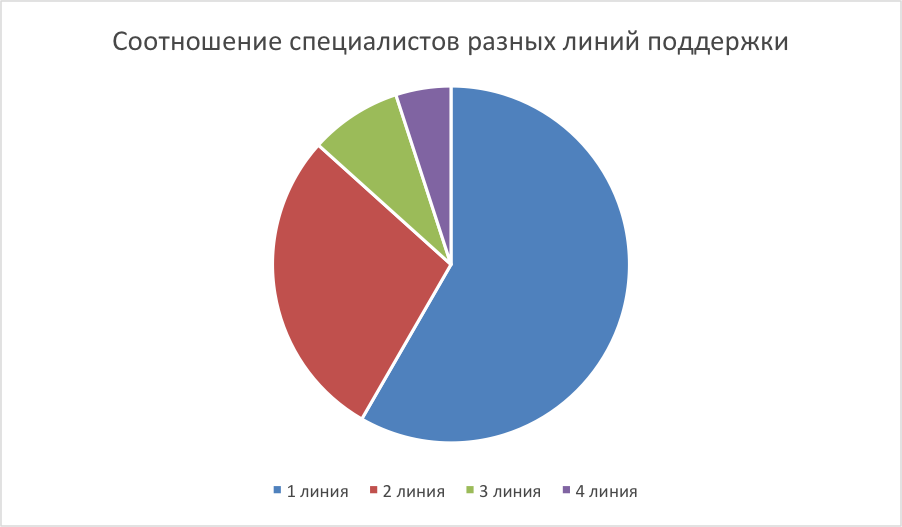
\includegraphics [scale=0.7] {ITSMTeamComposition}
  \caption{Диаграмма состава команд} 
  \label{img:ITSMTeamComposition}  
\end{figure}

Работа специалистов первой линии поддержки состоит из множества рутинных и простых задач. На рисунке \ref{img:EngineerTasks} показано соотношение разных типов проблем, встречающихся во время работы службы поддержки, в таблице \ref{IncidentDescription} приведена расшифровка типов. Данные подготовлены на основе анализа работы команд \icl.

\begin{figure} [h] 
  \center
  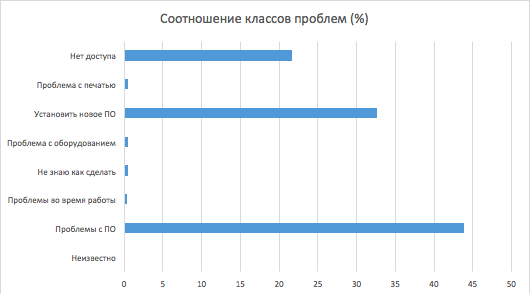
\includegraphics [scale=0.7] {EngineerTasks}
  \caption{Диаграмма соотношений типов проблем} 
  \label{img:EngineerTasks}  
\end{figure}

\begin{table} [htbp]
  \centering
  \parbox{15cm}{\caption{Категории инцидентов в области удаленной поддержки инфраструктуры}\label{IncidentDescription}}
%  \begin{center}
  \begin{tabular}{| p{7cm} || p{7cm} |}
 
  \hline
\textbf{Категория} & \textbf{Описание} \\
  \hline
Проблема с ПО	& Проблема при запуске ПО на компьютере. Решается переустановкой \\
  \hline
Проблемы во время работы  & Проблема с функционированием программного обеспечения\\
    \hline
Как сделать & Запрос на инструкцию по работе с тем или иным компонентом рабочей станции \\
      \hline
Проблема с оборудованием  & Неполадки на уровне оборудования \\
  \hline
Установить новое ПО       & Требование установки нового программного обеспечения \\
  \hline
Проблема с печатью        & Установка принтера в систему \\
    \hline
Нет доступа               & Нет доступа к общим ресурсам \\
  \hline
  \end{tabular}
%  \end{center}
\end{table}

Как показывают исследования, решение части задач может быть автоматизировано. Если это будет сделано,  специалисты получат дополнительное время для решения более сложных задач. \\

\textbf{Предпосылки развития изучаемой предметной области}. 
Основной тенденцией в развитии области удаленной поддержки инфраструктуры являются попытки удешевить и улучшить стоимость предоставления услуг \cite{OutsourceEff}. \par
Компании, работающие на этом рынке, вкладывают большие средства в автоматизацию. Кроме того, современное развитие науки и техники, точнее, вычислительных мощностей \cite{SuperComputer}позволяет провести автоматизацию даже самых наукоемких процессов. Дальнейшей перспективой развития области является замена человеческих специалистов автоматизированными системами. Разработки в этом направлении ведут многие компании, например, компания HP, которая имеет свою систему регистрации различных инцидентов и сейчас ведет работу над ее автоматизацией. В качестве некоторого сравнения можно провести параллель происходящего процесса с промышленной революцией XVIII–XIX веков (см., например, \cite{IndustrialRev}). \par

\textbf{Методологии, используемые в области ИТ-аутсорсинга: ITIL и ITSM}. \par
В области ИТ-аутсорсинга есть несколько готовых стандартов ведения работ, одним из которых является библиотека ITIL. Этот стандарт описывает лучшие практики организации работ в области ИТ-аутсорсинга. Используемый в библиотеке подход соответствует стандартам ISO 9000 (ГОСТ Р ИСО 9000) \cite{ITIL1} \cite{ITIL2} \cite{ITIL3}.
Наличие стандартов диктует унифицированность как постановки проблем, так и алгоритмов решения, а также способствует возможности частичной или в некоторых случаях полной автоматизации решения проблем. \par

\textbf{Оценка стоимости работы специалиста при автоматизации}.\par
По данным аналитики портала SuperJob \cite{SuperJob}], средняя зарплата системного администратора с опытом работы в Казани в 2014 году составляла 30 – 35 тыс. руб. 2014 года (из расчета на 1 час с учетом 21 рабочего дня в месяце~--- 179--208 руб. в час. В соответствии с действующим российским законодательством \cite{FiscalCodecs} расходы компании на одного работника определяются по формуле
\[
L = R + R*(F_1 +F_2+F_3),
\]
где R – выплата человеку в час, F1~--- НДФЛ 13\%, F2~--- совокупность отчислений в ФБ (6\%), ПФР (14\%), ТФОМС (2\%), ФФОМС (1,1\%), ФСС (2,9\%), F3~--- налог на прибыль (20\%). Таким образом, расходы компании на сотрудника варьируются от 285 до 314 руб. в час, а за 8-ми часовой рабочий день – от 2280 до 2512 руб. Далее, аренда выделенного сервера (Xeon X3, 1.7 GHz, 8GB RAM, 256GB SSD) стоит 8 900 руб./мес. (см. \cite{TimeWeb}) (53 рубля за 1 час с учетом 8-ми часового рабочего дня). Но сервер может работать 24 часа в сутки за исключением простоев на обслуживание, которые обычно составляют не более 5\% времени. Итого: сервер работает 478,8 часов в месяц. С этой точки зрения сервер будет стоить 18,5 руб. в час. Один сервер в своем быстродействии может заменить несколько специалистов при решении соответствующих задач. Чтобы решение было экономически эффективным, необходимо, чтобы оно сокращало расходы как минимум на 30\% (по данным \icl). Грубый подсчет на основе стоимости часа и пропорции показывает, что работа специалиста~--- это 6\% работы сервера (без учета работы сервера как несколько специалистов и примерно одинаковой скорости разрешения инцидентов). Таким образом уровень разрешения инцидентов системой в 50\% выполнит требования по прибыли примерно 186\%.

\textbf{Общая характеристика диссертации} 
\newcommand{\aim}{\textbf{Целью}}
\newcommand{\scope}{\textbf{Область исследования}}
\newcommand{\subject}{\textbf{Предметом исследования}}
\newcommand{\tasks}{задачи}
\newcommand{\defpositions}{\textbf{Основные положения, выносимые на~защиту:}}
\newcommand{\novelty}{\textbf{Научная новизна:}}
\newcommand{\influence}{\textbf{Практическая значимость}}
\newcommand{\reliability}{\textbf{Степень достоверности}}
\newcommand{\probation}{\textbf{Апробация работы.}}
\newcommand{\contribution}{\textbf{Личный вклад.}}
\newcommand{\publications}{\textbf{Публикации.}}

{\aim} работы является разработка интеллектуальной системы повышения эффективности деятельности ИТ-службы предприятия. \par
{\scope}~--- разработка методов и алгоритмов решения задач системного анализа, оптимизации, управления, принятия решений и обработки информации в ИТ-отрасли.\par
{\subject}  является процесс регистрации и устранения проблемных ситуаций, возникающих в ИТ-инфраструктуре предприятия.\par

Для достижения поставленной цели необходимо было решить следующие {\tasks}:
\begin{enumerate}
  \item Провести теоретико-множественный и теоретико-информационный анализ сложных систем в области поддержки информационной инфраструктуры;
  \item Создать модель целевой области;
  \item Исследовать модели мышления и выбрать наиболее подходящую;
  \item На основе выбранной модели мышления разработать модель проблемно-ориентированной системы управления, принятия решений и оптимизации процесса принятия, анализа и обработки запросов пользователя в области обслуживания информационной структуры предприятия;
  \item Создать архитектуру приложения на основе модели;
  \item Реализовать на основе этой архитектуры прототип интеллектуальной вопросно-ответной системы повышения эффективности деятельности ИТ-службы предприятия;
  \item Провести апробацию прототипа на тестовых данных.
\end{enumerate}

\defpositions
\begin{enumerate}
  \item Теоретико-множественный и теоретико-информационный анализ сложных систем в области поддержки информационной инфраструктуры;
  \item Построенная модель проблемно-ориентированной системы управления, принятия решений и оптимизации технических объектов в области обслуживания информационной инфраструктуры;
  \item Созданный прототип программной реализации модели проблемно-ориентированной системы управления, принятия решений и оптимизации обработки запросов пользователя в области обслуживания информационной инфраструктуры;
  \item Апробация прототипа проблемно-ориентированной системы управления, принятия решений и оптимизации деятельности на контрольных примерах и анализ ее результатов.
\end{enumerate}

\novelty проведенного исследования состоит в следующем:
\begin{enumerate}
  \item Создана модель проблемно-ориентированной системы управления, принятия решений в области обслуживания информационной структуры предприятия на основе модели мышления;
  \item Представлены новая модель данных для модели мышления и оригинальный способ хранения для этой модели, эффективный по сравнению с другими базами данных;
  \item Выполнено оригинальное исследование моделей мышления применительно к области обслуживания информационной структуры предприятия;
  \item На основе модели мышления Мински созданы архитектура системы обслуживания информационной структуры предприятия и программный прототип этой системы.
\end{enumerate}

\influence\ 
Система, разработанная в рамках данной диссертации носит значимый практический характер. Идея работы зародилась под влиянием производственных проблем в ИТ-отрасли, с которыми автор сталкивался каждый день в процессе разрешения различных инцидентов, возникающих в деятельности службы технической поддержки \icl~--- одном из крупнейших системообразующих предприятий ИТ-области Республике Татарстан. Поэтому было необходимо выработать глубокое понимание конкретной предметной области, чтобы выбрать приемлемое решение, получившее практическое применение в работе на проекте поддержки крупной сети продуктовых магазинов. \par
\reliability\ научных исследований и практических рекомендаций
базируется на корректной постановке общих и частных рассматриваемых задач,  использовании известных фундаментальных теоретических положений системного анализа, достаточном объёме данных, использованных при статистическом моделировании, и широком экспериментальном материале, использованном для численных оценок достижимых качественных показателей. \par 
Исследования, проведенные в диссертации, соответствуют паспорту специальности 05.13.01~--- Системный анализ, управление и обработка информации, сопоставление приведено в таблице \ref{ResearchDescription}.

\begin{longtable}{|p{7cm}|p{9cm}|}
 \caption[Сопоставление направлений исследований в рамках специальности 05.13.01 и исследований, проведенных в диссертации]{Сопоставление направлений исследований в рамках специальности 05.13.01 и исследований, проведенных в диссертации}\label{ResearchDescription} \\ 
 \hline
 
 \multicolumn{1}{|c|}{\textbf{Направление исследования}} & \multicolumn{1}{c|}{\textbf{Результат работы}}  \\ \hline 
\endfirsthead
\multicolumn{2}{c}%
{{\bfseries \tablename\ \thetable{} -- продолжение}} \\
\hline \multicolumn{1}{|c|}{\textbf{Направление исследования}} &
\multicolumn{1}{c|}{\textbf{Результат работы}}  \\ \hline 
\endhead

\hline \multicolumn{2}{|r|}{{Продолжение следует}} \\ \hline
\endfoot

\hline \hline
\endlastfoot
\hline
   Разработка критериев и моделей описания и оценки эффективности решения задач системного анализа, оптимизации, управления, принятия решений и обработки информации & В рамках работы была разработана модель системы принятия решения и обработки информации в области решения запросов пользователя на естественном языке. \\
   \hline
   Разработка проблемно-ориентированных систем управления, принятия решений и оптимизации технических объектов & По модели, разработанной в предыдущем пункте был разработан прототип системы принятия решения Thinking Understanding, который был испытан на модельных данных.\\
   \hline
   Методы получения, анализа и обработки экспертной информации & В рамках системы TU был разработан метод обработки экспертной информации - обучение при помощи модели мышления TU, основанной на принципах модели 6-ти Марвина Мински. \\
   \hline
   Разработка специального математического и алгоритмического обеспечения систем анализа, оптимизации, управления, принятия решений и обработки информации & В рамках разработки системы TU были созданы специальные алгоритмы для анализа запросов пользователя и принятия решений.\\
  \hline 
  Теоретико-множественный и теоретико-информационный анализ сложных систем & В рамках работы был проведен комплексный анализ области поддержки программного обеспечения, с помощью которого была построена система данной области и выделены участки для оптимизации принятия решений.\\
  \hline
  Методы и алгоритмы интеллектуальной поддержки при принятии управленческих решений в технических системах & Система, разработанная в рамках данной работы в включает в себя инновационные методы и алгоритмы поддержки принятия решений, использующих в своей основе модель мышления на базе модели мышления Человека, описанной в книге Марвина Мински. \\ 
  \hline
  Визуализация, трансформация и анализ информации на основе компьютерных методов обработки информации & Представлена наглядная визуализация данных по системному анализу области удаленной поддержки инфраструктуры. \\
  \hline	
\end{longtable}


\probation\
 Основные результаты диссертационной работы докладывались на следующих конференциях:
\begin{itemize}
	\item Десятая молодежная научная школа-конференция "Лобачевские чтения~---2011. Казань, 31 октября~--4 ноября 2011";
	\item 3rd World Conference on Information Technology (WCIT-2012); 
	\item Искусственный интеллект и естественный язык (AINL-2013);
	\item Электронная Казань~--- 2014;
	\item Электронные библиотеки: перспективные методы и технологии, электронные коллекции (RCDL-2014);
	\item Agents and multi-agent systems: technologies and applications (AMSTA-2015).
\end{itemize}
Практическая апробация результатов работы проводилась на выгрузке инцидентов из системы регистрации запросов службы технической поддержки ИТ-инфраструктуры \icl. Созданная система показала требуемые результаты (процент успешно обработанных запросов более чем 30\%) обработки данной информации.
\contribution\ Автор исследовал целевую область: проводил анализ запросов пользователей и классифицировал их, вместе с Талановым Максимом Олеговичем изучал модель мышления Марвина Мински; создавал базовую архитектуру систему; вместе с Талановым Максимом Олеговичем проводил разработку компонентов модели, адаптируя теорию Марвина Мински. Автор проводил испытание системы на целевых запросах; отлаживал работу системы.
\publications\ Основные результаты по теме диссертации изложены в 9 печатных изданиях  \cite{Lobachevskii},\cite{WCIT-2012},\cite{AINL-2013},\cite{ISGZ}, \cite{IJSE-1}, \cite{IJSE-2}, \cite{RCDL-2014}, \cite{AMSTA-2015}, \cite{VAK-1}, из которых статьи \cite{RCDL-2014},\cite{AMSTA-2015} проиндексированы в БД Scopus, статья \cite{AMSTA-2015} проиндексирована в БД Web Of Science, работа \cite{VAK-1} опубликована в журнале из списка ВАК, статья  \cite{ISGZ} проиндексирована в БД РИНЦ, работы \cite{Lobachevskii},\cite{WCIT-2012},\cite{AINL-2013},\cite{ISGZ} опубликованы в материалах международных и всероссийских конференций.



 % Характеристика работы по структуре во введении и в автореферате не отличается (ГОСТ Р 7.0.11, пункты 5.3.1 и 9.2.1), потому её загружаем из одного и того же внешнего файла, предварительно задав форму выделения некоторым параметрам
%% регистрируем счётчики в системе totcounter
\regtotcounter{totalcount@figure}
\regtotcounter{totalcount@table}       % Если поставить в преамбуле то ошибка в числе таблиц
\regtotcounter{TotPages}               % Если поставить в преамбуле то ошибка в числе страниц

\textbf{Объем и структура работы.} Диссертация состоит из введения, четырех глав, заключения и пяти приложений. Полный объём диссертации составляет \formbytotal{TotPages}{страниц}{у}{ы}{} 
с~\formbytotal{totalcount@figure}{рисунк}{ом}{ами}{ами}
и~\formbytotal{totalcount@table}{таблиц}{ей}{ами}{ами}. Список литературы содержит  
\formbytotal{citenum}{наименован}{ие}{ия}{ий}.
\clearpage

    % Введение
\chapter{Интеллектуальные системы регистрации и анализа проблемных ситуаций, возникающих в ИТ-инфраструктуре предприятия} \label{chapt1}

\section{Сравнительный анализ систем регистрации и устранения проблемных ситуаций} 
В данной главе рассматриваются имеющиеся на данный момент интеллектуальные системы регистрации и анализа проблемных ситуаций. \par
\textbf{HP OpenView} \cite{HPOpenView} \cite{HP1} \cite{HP2} \cite{HP3} является комплексным программным решением по мониторингу ИТ-инфраструктуры предприятия и имеет множество модулей. На рисунке \ref{img:hpopenview} представлен вид системы, которая обладает широким спектром возможностей: мониторинг \cite{HP4} \cite{HP5}; регистрация инцидентов; управление системами. Система не поддерживает: понимание и формализацию запросов; автоматическое исправление проблемы на основе формализации запроса.

\begin{figure} [h] 
  \center
  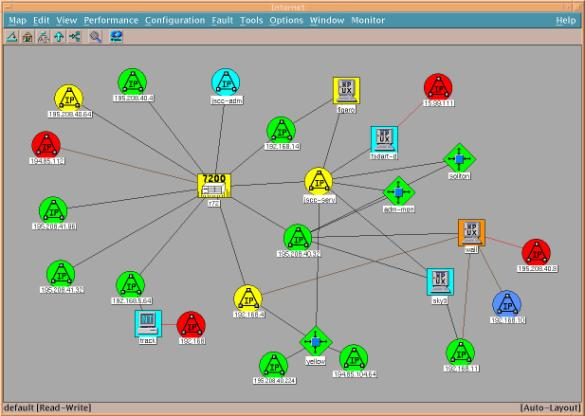
\includegraphics [scale=1.0] {hpopenview}
  \caption{HP OpenView} 
  \label{img:hpopenview}  
\end{figure}

Система \textbf{ServiceNOW}~--- средства автоматизации сервиса. На рисунке \ref{img:svnow} представлен вид этой системы, которая предоставляет следующие возможности: регистрация инцидентов и создание цепи их обработки. Система не поддерживает: понимание и формализацию запросов; автоматическое исправление проблемы на основе формализации запроса. Система широко используется в ИТ-инфраструктуре CERN \cite{SN1} \cite{SN2} для регистрации инцидентов и их решения.

\begin{figure} [h] 
  \center
  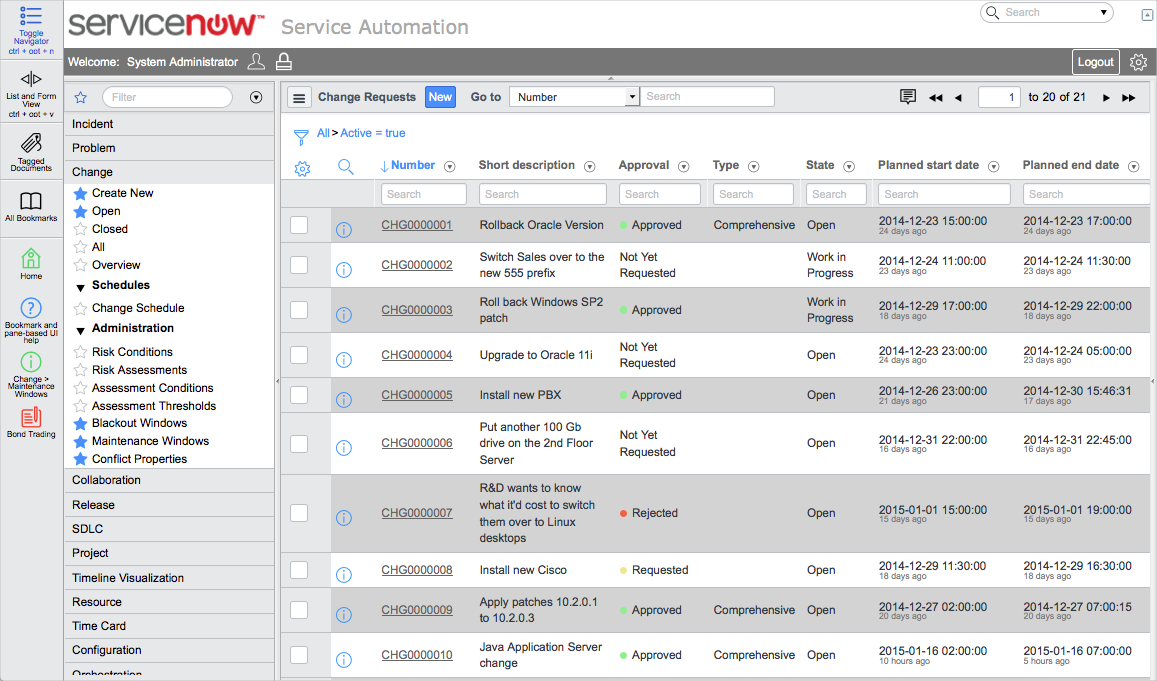
\includegraphics [scale=0.3] {svnow}
  \caption{Service NOW} 
  \label{img:svnow}  
\end{figure}

\textbf{IBMWatson}~--- это вопросно-ответная система, которая поддерживает: понимание и формализацию запросов и поиск решений. Система не поддерживает автоматическое исправление проблемы на основе формализации запроса. Система широко используется в медицине для постановки диагнозов болезней \cite{IBM1} \cite{IBM2} \cite{IBM3} \cite{IBM4} и реализует базовые принципы искусственного интеллекта \cite{IBM5} \cite{IBM6}. Ее разработка велась под суперкомпьютер IBM Deep Blue \cite{IBM7}. На рисунке \ref{img:Watson-Analytics} представлен общий вид этой системы. \par


\begin{figure} [h] 
  \center
  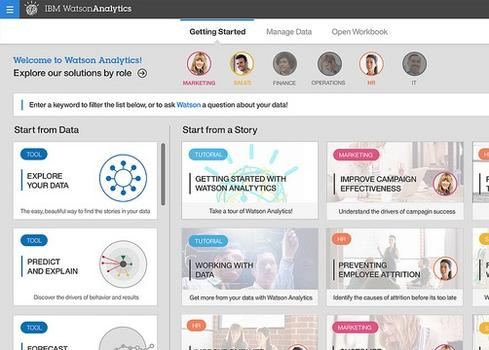
\includegraphics [scale=1.0] {Watson-Analytics}
  \caption{Пример работы системы Watson} 
  \label{img:Watson-Analytics}  
\end{figure}

Кроме того, известны следующие дополнительные способы и системы автоматизации:
\begin{itemize}
	\item Обработка инцидентов посредством регулярных выражений. В таком решении нет гибкости, так как обработка идет путем поиска ключевых слов вне контекста. Метод регулярных выражений частично используется для обработки естественного языка, поиска  \cite{REG1}, диагностики активных систем \cite{REG2}, анализа поведения функций \cite{REG4}, обработки данных в системе eDiscovery \cite{REG5}, в разработке способах программирования \cite{REG3};
	\item Обработка инцидентов при помощи скриптов~--- автоматизируются лишь рутинные операции.
\end{itemize} \par
Таким образом, был сформирован список требований к системе, которые в следующем разделе будут уточнены и формализованы.  На данный момент ни одна из исследованных систем в полной мере автоматически не решает запросы пользователей: фиксирует их, проводит анализ, ищет решение, применяет решение и дает обратную связь пользователю. Каждая система в той или иной мере реализует те или иные критерии, но системы, которая отвечает всем критериям нет. 

\section{Основные требования к интеллектуальным системам регистрации и анализа проблемных ситуаций в ИТ-области} \label{sect3_2}
Для того чтобы создать модель системы необходимо определить требования к ней, или критерии, соответствие которым будет служить одним из доказательств состоятельности системы наряду с экспериментальными результатами. \par

Перечисленные ниже требования сформированы, исходя из возможностей специалистов поддержки, а также анализа проблем, которыми они занимаются. Большинство инцидентов – тривиальные и типичные, но все они разные. Для человека проблемы ”Please install Firefox” и ”Please install Chrome” идентичны, но с точки зрения формализации это не так~--- общее в них можно найти, взглянув на генерализацию различающейся части: Firefox и Chrome являются пакетами программного обеспечения. \par
Итак, основными требованиями к интеллектуальным системам регистрации и анализа проблемных ситуаций в ИТ-области являются возможности реализации этими системами: мониторинга ИТ-инфраструктуры пользователя; регистрации инцидентов; создания цепи обработки (Workflow) инцидента; понимания и формализации запросов на естественном языке; поиска решений и применения найденных решений; обучения решению инцидента; умения проводить логические рассуждения (генерализацию, специализацию, синонимичный поиск). \par
Из всего списка требований к системе важно выделить формализацию запросов на естественном языке. Это отдельная и обширная область исследования. Ниже приведены результаты анализа разработок в данной области. 

\clearpage

\section{Сравнительный анализ методов и комплексов обработки текстов на естественном языке}


\subsection{Обработка эталонных текстов} \label{sect2_1}
В данном разделе проведен обзор обработчиков естественного языка. За основу были взяты инциденты, выгруженные из систем поддержки ИТ-инфраструктуры \icl. Ввиду специфики предметной области (информационные технологии) основным языком был выбран английский язык. Был сформирован список из типичных эталонных фраз, на которых тестировались обработчики естественного языка. Фразы были выявлены путем анализа существующих отчетов об инцидентах. Примерами инцидентов являются следующие запросы.\par
\textbf{Инцидент 1}.
\textit{
User had received wrong application. User has ordered Wordfinder Business Economical for her service tag 7Q4TC3J, there is completed order in LOT with number ITCOORD-18125. However she received wrong version, she received Wordfinder Tehcnical instead of Business Economical. Please assist.
}\par
\textbf{Инцидент 2}.
\textit{
Laptop – user has almost full C:\ but when he looks in the properties of the files and folders on C:\ they are only 40GB and he has a 55GB drive.
}\par
\textbf{Инцидент 3}.
\textit{
User cannot find Produkt Manageron start menu. Please reinstall. 
}\par
\textbf{Инцидент 4}.
\textit{
User needs to have pdf 995 re-installed please.
}\par

При анализе были использованы следующие обработчики естественного языка: Open NLP \cite{OpenNLP}, Relex\cite{OpenCogRelex}, StanfordParser \cite{StanfordParser}. Результат их работы оценивался при помощи метрик, представленных в таблице \ref{Metrics}, а полученные результаты приведены на рисунке \ref{img:ParserComp}. 

\begin{table} [htbp]
  \centering
  \parbox{15cm}{\caption{Таблица метрик}\label{Metrics}}
%  \begin{center}
  \begin{tabular}{| p{5cm} |p{5cm}| p{5cm} |}
  
  \hline
Метрика & Описание & Формула \\
  \hline
 
Precision	& Точность & 
$$ 
P=\frac{tp}{tp+fp}
$$ где P~--- precision, tp~---  успешно обработанные, fp~--- ложно успешные \\
 \hline
Recall	& Чувствительность & 
$$ 
R=\frac{tp}{tp+fn}
$$ где R~--- recall, tp~--- успешно обработанные, fn~--- ложно неуспешные \\
 \hline
F	& F-measure (результативность) & 
$$ 
F=\frac{P*R}{P+R}
$$ Где P~--- precision, R~--- recall.   \\
 \hline
  \end{tabular}
%  \end{center}
\end{table}

\begin{figure} [h] 
  \center
  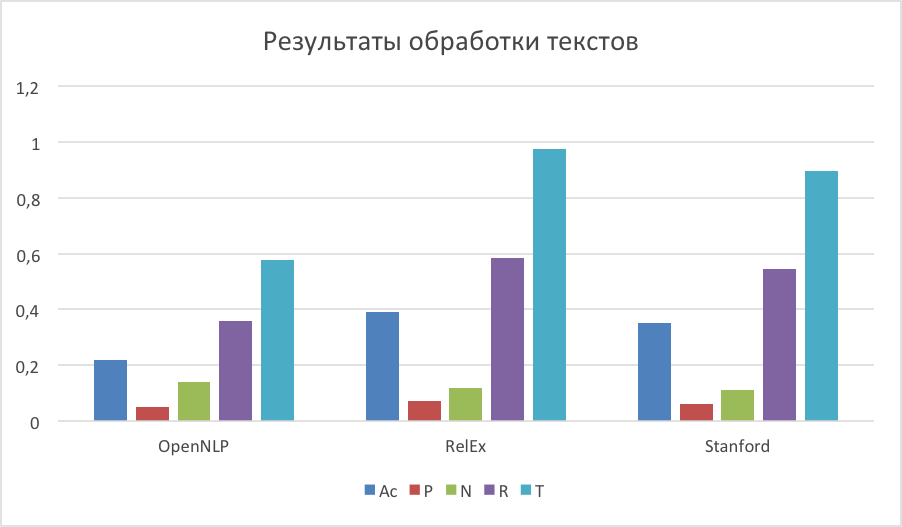
\includegraphics [scale=0.8] {ParserCompare}
  \caption{Результаты обработки текстов} 
  \label{img:ParserComp}  
\end{figure}

Из диаграммы видно, что наилучшее результаты показывает обработчик Relex\cite{OpenCogRelex}. После анализа необработанных инцидентов у всех обработчиков было выявлены проблемы двух типов:
\begin{enumerate}
	\item невозможность корректировки простых грамматических ошибок, связанных с пропущенными пробелами или неверным форматированием (ошибки первого типа);
	\item неверная интерпретация слов в предложении, например, слово please интерпретировалось как глагол, хотя является по смыслу "формой вежливости" (ошибки второго типа).
\end{enumerate}	\par

Несмотря на хорошие результаты~--- 63\% успешно разобранных предложений, ошибки первого и второго типа серьезно ухудшают результат. Эффективность разбора предложений в 63\% недостаточна для успешной работы системы. Чтобы улучшить показатель, был создан комплекс мер для устранения ошибок первого и второго типа.
	
 
\clearpage
\subsection{Исправление ошибок первого и второго типа} \label{sect2_2}
Чтобы исправить проблемы, связанные с ошибками первого и второго типа, была введена предварительная обработка текста, состоящая из 2-х фаз: комплексная корректировка для ошибок первого типа; обработка при помощи внутренней базы знаний для ошибок второго типа. 
Чтобы избавиться от орфографических, грамматических и синтаксических ошибок, был сконструирован составной корректировщик, который имеет модульную структуру и осуществляет корректировку последовательно (рис. 1.5). В результаты были сконструированы модули корректировки: Google API~--- модуль подключения к открытым системам Google для использования их алгоритмов корректировки; After the Deadline~--- модуль, использующий открытый программный продукт After the Deadline для исправления текстов; 

Таким способом удалось исправить большинство ошибок, связанный с синтаксисом, грамматикой и орфографией. Также удалось исправить ошибки неверного написания: наличия лишних пробелов, пропуска запятых и точек. Но по-прежнему осталась проблема обработки неверной интерпретации слов в тексте. \par

Для корректировки ошибок второго типа был сконструирован модуль для обработчика естественного языка Relex, который разбивал стандартный процесс обработки на «предобработку» и «обработку». Стадия «обработки» включает в себя алгоритм работы такой же как был до этого в модули, а стадия «предобработки» проверяет входные данные (слово или предложение) на предмет его вхождения во внутреннюю базу знаний и если таковое имеется, то приложение передает соответствующие корректировки обратно в модуль. Например, Relex во фразе "please install firefox" считает, что "please"~--- это глагол, поэтому базе знаний нашей системы отмечено, что "please"~--- это форма вежливости, тем самым Relex больше не интерпретирует "please" как глагол.

\clearpage
\subsection{Сравнение средств обработки русского и английского языков} \label{sect2_3}
Средства обработки естественного языка принято относить к большому классу средств NLP – Natural Language Processing \cite{NLP}. Для английского языка существует множество открытых средств обработки естественного языка, для русского языка найти их гораздо сложнее. Рассмотрим архитектуру средств обработки естественного языка на примере OpenCog Relex. \par
OpenCog Relex использует результаты работы открытого компонента для лексического анализа под названием Link Grammar \cite{linkgrammar}. Он поддерживает множество языков: английский, русский, турецкий, немецкий и т.д.  В качестве формата вывода Relex использует синтаксис Link Grammar и преобразует его в формат связей, как показано в примере 1. Разбор примера приводится далее. 

\textbf{Пример 1}. User is unable to start KDP web, please reinstall Java.\\
\textbf{Результат} 
\begin{verbatim}
		_obj(start, KBP)
pos(start, verb)
inflection-TAG(start, .v)
tense(start, present)
pos([web], WORD)
noun_number(KBP, singular)
definite-FLAG(KBP, T)
pos(KBP, noun)
_advmod(reinstall, please)
pos(reinstall, verb)
inflection-TAG(reinstall, .v)
tense(reinstall, present)
pos(please, adv)
inflection-TAG(please, .e)
noun_number(Java, singular)
definite-FLAG(Java, T)
pos(Java, noun)
pos(., punctuation)
_obj(,, Java)
pos(,, verb)
tense(,, infinitive)
HYP(,, T)
_to-do(unable, ,)
pos(unable, adj)
inflection-TAG(unable, .a)
tense(unable, present)
pos(to, prep)
inflection-TAG(to, .r)
pos(be, verb)
inflection-TAG(be, .v)
_predadj(User, unable)
noun_number(User, singular)
definite-FLAG(User, T)
pos(User, noun)

\end{verbatim}



Далее возьмем разбор слова start. В результате мы получаем несколько отношений:
\begin{itemize}
	\item pos(start, verb) - start глагол
	\item tense(start, present) - время настоящее
	\item inflection-TAG(start, .v) -  метод обозначения на схеме (индекс)
\end{itemize} \par
Остальные обработчики пока не поддерживают русский язык. Существуют открытые проекты, но они еще недостаточно развиты.
\section{Выводы}
В данной главе были рассмотрены существующие на данный момент интеллектуальные системы регистрации и анализа проблемных ситуаций, возникающих в ИТ-инфраструктуре предприятия.
 В таблице \ref{Comparsion} приведены сводные данные по системам. В главе также выработаны критерии сравнения обработчиков естественного языка и выполнен основной анализ обработчиков естественного языка. По показателям эффективности было решено использовать OpenCog Relex.

\begin{longtable}{|p{6cm}|p{0.5cm}|p{0.5cm}|p{0.5cm}|}
 \caption[Сравнительный анализ существующих решений]{Сравнительный анализ существующих решений}\label{Comparsion} \\ 
 \hline
 
 \multicolumn{1}{|c|}{\textbf{Сравнительный пункт}} & \multicolumn{1}{c|}{\textbf{HP Open View}} & \multicolumn{1}{c|}{\textbf{ServiceNOW}} & \multicolumn{1}{c|}{\textbf{IBM Watson}} \\ \hline 
\endfirsthead
\multicolumn{2}{c}%
{{\bfseries \tablename\ \thetable{} -- продолжение}} \\
\hline \multicolumn{1}{|c|}{\textbf{Сравнительный пункт}} & \multicolumn{1}{c|}{\textbf{HP Open View}} & \multicolumn{1}{c|}{\textbf{ServiceNOW}} & \multicolumn{1}{c|}{\textbf{IBM Watson}}  \\ \hline 
\endhead

\hline \multicolumn{2}{|r|}{{Продолжение следует}} \\ \hline
\endfoot

\hline \hline
\endlastfoot
\hline
   Мониторинг & Да & Да & Да \\
   \hline
   Регистрация инцидентов & Да & Да & Да\\
   \hline
   Управление системами & Да & Нет & Нет \\
   \hline 
   Создание цепи обработки (Workflow) инцидента & Да & Да & Нет \\
   \hline 
   Понимания и формализацию запросов на естественном языке & Нет & Нет & Да \\
   \hline 
   Поиск решений & Нет & Нет & Да \\
   \hline 
   Применение решений & Нет & Нет & Нет \\
   \hline
   Обучение решению инцидента & Нет & Нет & Да \\
   \hline
   Умение проводить логические рассуждения: генерализацию, специализацию, синонимичный поиск & Нет & Нет & Нет \\
   \hline
   
\end{longtable}
\clearpage
           % Глава 1
\chapter{Модель интеллектуальной системы принятия решений для регистрации и анализа проблемных ситуаций в ИТ-инфраструктуре предприятия} \label{chapt3}

В данной главе рассматриваются модели, которые были изучены и использованы при создании системы принятия решений для регистрации и анализа проблемных ситуаций в ИТ-инфраструктуре предприятия. Отметим, что работа над системой велась с 2011 года, за истекшее время было создано три рабочих версии прототипа системы, реализующих различные модели мышления. \par
Созданными и испытанными моделями, использованными при создании системы принятия решений для регистрации и анализа проблемных ситуаций в ИТ-инфраструктуре предприятия, являются:
 \begin{itemize}
	\item модель Menta 0.1, построенная с использованием деревьев принятия решений;
	\item модель Menta 0.3, построенная с использованием генетических алгоритмов \cite{ArtificialIntelligence} ;
	\item модель TU 1.0, основанная на модели мышления Марвина Мински  \cite{EmotionMachine}.
\end{itemize}

Модель, построенная на базе нейронных сетей (поддерживающая обучение) была отброшена на предварительной стадии оценки, так как она предъявляет большие требования к производительности \cite{NEURAL}, что в свою очередь порождает высокую стоимость. Далее каждая модель будет рассмотрена подробно.

%====================

%====================
\section{Построение модели Menta 0.1 с использованием деревьев принятия решений} \label{sect3_1}
Данная модель являлась одной из первых, которые были опробована. Она основана на деревьях принятия решений \cite{DTREE}, которые широко используются в вопросно-ответных системах \cite{DC1}, \cite{DC2}, \cite{DC3}. При построении модели использовались следующие компоненты: обработка запросов на естественном языке; поиск решения; применение найденного решения; база знаний.\par
Система ориентирована на выполнение таких простых команд, как, например, "Добавить поле на форму". Основные функции модели представлены следующими потоками: получение и формализация запроса; поиск решения при помощи деревьев принятия решений; изменение приложения, согласно запросу; генерация и компиляция приложения. Рассмотрим подробнее как устроена система. Начнем с того, как представлены данные в системе.

\subsection{База знаний на основе OWL}
В качестве представления данных в системе использовалась база знаний на основе OWL-файла (см. \cite{OWL}). С помощью редактора Protege \cite{Protege} в базу вводились начальные данные о целевом приложении (приложение, которое будет модифицироваться системой согласно запросам от пользователей) в виде семантической сети. В качестве такого приложения была создана простая программа, которая вела учет заказов на покупку книг от пользователя. \par

 На рисунке \ref{img:order-owl} представлен один из классов этой программы~--- Order~--- в формате OWL. Этот класс отвечает за обработку заказов. Слева отображены супер классы (классы-предки), к которым он привязан. Например, класс BLL относится к бизнес-логике приложения, Module~--- отдельный модуль в рамках системы. Справа представлены свойства класса, а их описания приведены в таблице \ref{OrderPropertyDescription}. С помощью предикатов определяется поведение свойства: создать файл, создать новое поле. В таблице \ref{Predicates} представлено описание иерархии предикатов. На рисунке \ref{img:CreateCustomer} представлен класс CreateCustomer в OWL. Сюда входит описание всех необходимых свойств для генерации файла исходного кода на языке Java.

\begin{figure} [h] 
  \center
  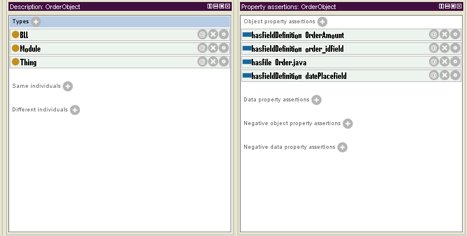
\includegraphics [scale=0.7] {OrderOWL}
  \caption{Представление класса Order в OWL. Визуализация Protege.} 
  \label{img:order-owl}  
\end{figure}

\clearpage
\begin{table} [htbp]
  \centering
  \parbox{15cm}{\caption{Описание свойств класса Order в OWL}\label{OrderPropertyDescription}}
%  \begin{center}
  \begin{tabular}{| p{3cm} | p{4cm} | p{8cm} |}
  \hline
 \textbf{Свойство} & \textbf{Предикат} & \textbf{Описание} \\
  \hline
    OrderAmount	& hasFieldDefinition & Поле: сумма заказа \\
  \hline
orderidField	& hasFieldDefinition & Поле: идентификатор заказа \\
  \hline
Order.java	& hasFile & Идентификатор имени файла для генерации \\
  \hline
datePlaceField	& hasFieldDefinition & Поле: время размещения заказа \\
  \hline
    \end{tabular}
%  \end{center}
\end{table}

\begin{table} [htbp]
  \centering
  \parbox{15cm}{\caption{Описание иерархии предикатов}\label{Predicates}}
%  \begin{center}
  \begin{tabular}{| p{7cm} | p{8cm} |}
  \hline
  
\textbf{Предикат} & \textbf{Описание} \\
  
    \hline
 hasFieldDefinition & Предикат, обозначающий свойство класса \\
  \hline
 hasMethodDefinition & Предикат, обозначающий функцию \\
  \hline
classDefinition & Обозначение класса \\
  \hline
database & Обозначение базы данных\\
  \hline
    \end{tabular}
%  \end{center}
\end{table}

\begin{figure} [h] 
  \center
  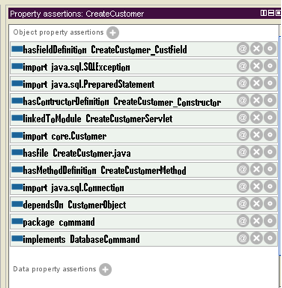
\includegraphics [scale=0.6] {CreateCustomer}
  \caption{Представление класса CreateCustiner в OWL. Визуализация Protege.} 
  \label{img:CreateCustomer}  
\end{figure}
\clearpage
\subsection{Основные компоненты модели}
Основными компонентами модели являются: Request parser (Stanford parser); Генерация Action (Action Generator); Исполнение Action (Action Applier); Генерация приложения (Application Generator). \par
\emph{Request parser} формализует запрос на естественном языке. \emph{Action Generator} генерирует Action объект из результатов работы парсера, основываясь на Деревьях принятия решений \cite{DCFOREST} и базе данных. Основной задачей данного модуля является генерация имени, действия и поля. Модуль \emph{Action Applier} отыскивает объект в модели по данным от Action Generator и производит действие, кроме того, используя предикат dependOn, он производит модификацию всех зависимых классов. \par
 В модели поддерживается два типа Action: RemoveFieldAction (удаление поля), AddFieldAction(добавление поля). После завершения работы производится генерация целевого приложения на языке Java при помощи OWL модели в модуле \emph{Application Generator}. На рисунке \ref{img:MentaUseCase} представлена UML диаграмма последовательности для основного рабочего потока приложения: пользователь вводит в систему запрос "Add new field to customer"; модуль StanfordParser вычлиняет из запроса связи типа dobj (связь объекта и действия); модуль ActionGenerator создает на основе связей действие; модуль ActionApplier, используя действие изменяет модель приложения; модуль ApplicationGenerator применяет изменения к приложению. В результате у класса Customer (представляет клиента магазина в приложении) появляется новое поле "New". \par
\begin{figure} [h] 
  \center
  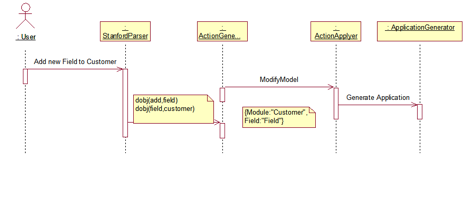
\includegraphics [scale=1.0] {MentaUseCase}
  \caption{UML диаграмма последовательности для основного потока в модели Menta 0.1} 
  \label{img:MentaUseCase}  
\end{figure}
После проведения экспериментов было выявлено, что приложение не может использовать ранее найденные решения, абстрагируя их, например, система знает как произвести операцию добавления поля, но вот подобную операцию~--- добавить метод~--- сделать не может. Поиск решения также требовал специального обучения: система не могла путем перебора информации в своей базе знаний найти решение.  В системе также не было возможности обучения. \par
После анализа ошибок была предпринята попытка найти более универсальное решение. Результатом стало построение Menta 0.3, описанной ниже.

%===============================
\section{Модель Menta 0.3 с использованием генетических алгоритмов} \label{chapt2}
В данную модель по сравнению с предыдущей были добавлены модуль логики для оценки решения и модуль генетических алгоритмов для генерации решения. Отметим, что генетические алгоритмы часто применяются в биологически инспирированных системах \cite{G1}, \cite{G3}. Кроме того, есть примеры их использования и в системах поддержки принятия решений, однако эффективность таких систем не подтверждена \cite{G2}. В рамках модели Menta 0.3 были отработаны следующие основные компоненты будущей итоговой модели: критерии приемки (Acceptance Criteria); How-To~--- для хранения решений проанализированных проблем; формат данных OWL; использование логических вычислений для проверки решения. Система Menta 0.3 содержала внутри себя модель целевого приложения (как и Menta 0.1) и список решений тех или иных проблем (How-To). При помощи генетического алгоритма модель строила How-To решение проверяла его при помощи логического движка NARS \cite{NARS} на соответствие входным критериям приемки. С точки зрения генетических алгоритмов это~--- функция отбора особей из поколения \cite{GFITNESS}. 

\subsection{Основные компоненты модели}
Модель состоит из компонентов, представленных в Таблице \ref{ModulesMenta03}.

\begin{longtable}{|p{5cm}|p{11cm}|}
 \caption[Компонетны модели Menta 0.3]{Компонетны модели Menta 0.3}\label{ModulesMenta03} \\ 
 \hline
 
 \multicolumn{1}{|c|}{\textbf{Компонент}} & \multicolumn{1}{c|}{\textbf{Описание}}  \\ \hline 
\endfirsthead
\multicolumn{2}{c}%
{{\bfseries \tablename\ \thetable{} -- продолжение}} \\
\hline \multicolumn{1}{|c|}{\textbf{Компонент}} &
\multicolumn{1}{c|}{\textbf{Описание}}  \\ \hline 
\endhead


\endfoot

\hline \hline
\endlastfoot
 MentaController & Веб-служба \cite{WebService}, который предоставляет интерфейс для общения с пользователем и остальными системами \\
  \hline
 SolutionGenerator & Модуль отвечает за генерацию решения. На вход он получает Acceptance Criteria. Основой является генетический алгоритм. Для него был выбран framework ecj \cite{ECJ} . Из всех возможных классов в базе знаний, отсеянных по классификатору составляются паросочетания. К каждому паросочетанию применяется логическое суждение на основе AcceptanceCriteria (за это отвечает модуль ReasonerAdapter). В итоге паросочетание получает оченку в виде пары Frequency, Confidence (частота, вероятность). 
Таким образом находится максимально лучше паросочетание. Если его показатель 1,1, то решение принимается, иначе отбрасывается (на данный момент установлен жесткий показатель).
SolutionGenerator включает в себя SolutionChecker, который включает в себя ReasonerAdapter.
 \\
  \hline
SolutionChecker & Проверка решения. Принимает на вход выбранные How-To, AcceptanceCriteria. Комбинирует их и передает ReasonerAdapter. \\
  \hline
ReasonerAdapter & Транслирует  How-To в термины NARS. NARS – non-axiomatic reasoning system \cite{NARS}(система логических суждений, разработанная профессором Пеем Вонгом). Принцип действия NARS – это всевозможная комбинация фактов. Каждый факт имеет свои частоту и вероятность. Их сочетанием получается композиция данных фактов.\\
  \hline
  Translator & Транслирует объекты базы знаний (знания) в отчеты. Последние бывают следующих типов: Solution Report; UML Report; Patch. В данной версии используется первый тип отчета. Он содержит описание на выбранном языке программирования решения, найденного системой.\\
  \hline
  Applicator & Данный модуль применяет решение к модели приложения, содержащейся в базе знаний. Также данная модель включает FileApplicator, который генерирует решение в виде файлов на выбранном языке программирования. \\
  \hline
  KBServer & База знаний приложения. Используется сервер non-SQL БД HypergraphDB. \\
  \hline
%  \end{center}
\end{longtable}
В предыдущей модели в качестве хранения данных использовался в файл, что было неудобно в случае, если приложение работает параллельно над несколькими запросами. В системе Menta 0.3 стал использоваться специальный сервер баз данных, речь о котором пойдет далее.

\subsection{База знаний на основе графов}
При реализации KBServer был создан промежуточный слой DAO (Data Access Object), данный подход широко используется в проектировании программного обеспечения \cite{THREELAYERARCH}. Это позволяет максимально отделить реализацию KBServer от конкретного хранилища. \par 

\textbf{EntityManagerFactory}. Данный класс является входной точкой и создает объект, с помощью которого приложение осуществляет работу с базой знаний. Класс автоматически выбирает необходимые настройки для объекта. \par

\textbf{EntityManager}. Это основной класс для загрузки, хранения объектов из базы данных.\par

\textbf{Configuration}. Этот класс хранит параметры настройки базы данных, такие как физическое положение БД и максимальное количество подключений. \par 
\textbf{EntityTransaction}. Данный класс используется для управления транзакциями при доступе к объектам базы данных. \par
При выборе физического хранилища данных были проанализированы несколько хранилищ OWL-данных: OWLIM, SESAME и HG. Результаты их сравнения представлены в таблице \ref{DatabaseEngineComparison}.
\begin{longtable}{|p{6cm}|p{3cm}|p{3cm}|p{3cm}|}
 \caption[Сравнение скорости доступа к данным баз знаний]{Сравнение скорости доступа к данным баз знаний}\label{DatabaseEngineComparison} \\ 
 \hline
 
 \multicolumn{1}{|c|}{\textbf{}} & \multicolumn{1}{c|}{\textbf{Sesame}} & \multicolumn{1}{c|}{\textbf{OWLIM}} & \multicolumn{1}{c|}{\textbf{HG}} \\ \hline 
\endfirsthead
\multicolumn{2}{c}%
{{\bfseries \tablename\ \thetable{} -- продолжение}} \\
\hline \multicolumn{1}{|c|}{\textbf{}} & \multicolumn{1}{c|}{\textbf{Sesame}} & \multicolumn{1}{c|}{\textbf{OWLIM}} & \multicolumn{1}{c|}{\textbf{HG}} \\ \hline 
\endhead

\endfoot

\hline \hline
\endlastfoot
 \textbf{Единицы измерения} & \textbf{мс.} & \textbf{мс.} & \textbf{мс.} \\
  \hline
 предварительно скомпилированные запросы & 26 253 & 3 012 & 6 813 \\
  \hline
 без кеша & 30 545 & 1 122 & 9 045 \\
  \hline
 с кешем & 24 258 & 962 & 985 \\
%  \end{center}
\end{longtable}

Несмотря на то, что OWLIM дает лучшее результаты, был выбран HGDB, так как HGDB предоставляет более широкие возможности доступа к данным, такие, например, как поддержка алгоритмов работы с графами.

%========================================
%========================================

\section{Модель TU 1.0, основанная на модели мышления Марвина Мински}
Следующим этапом разработки стала модель, построенная с применением теории Марвина Мински. Эта модель сохранила следующие основные концептуальные элементы предыдущих моделей и показала свою состоятельность на контрольных примерах: Acceptance Criteria; Обучение; Поиск и применение решения; Отсутсвие обработки естественного языка. Данная модель является более универсальной и представляет собой верхнеуровневую архитектуру обработки запроса (мышления), где компонентами являются лучшие части предыдущих систем.
\subsection{Особенности модели мышления}
В 2006 году Марвин Мински опубликовал свою книгу "The emotion machine" \cite{EmotionMachine}, в которой предложил свой взгляд на систему мышления и памяти человека. В основу теории легла парадигма триплета \triplet, k-line (линия, которая связывает приобретенные знаний, например, огонь~--- горячо) для сопоставления знаний. На рисунке \ref{img:csw} представлена схематичное изображение триплета \triplet. \par
\begin{figure} [h] 
  \center
  \includegraphics [scale=1.0] {CSW}
  \caption{\triplet} 
  \label{img:csw}  
\end{figure}

\textbf{Критик} представляет собой определенный переключатель: внешние обстоятельства, события или иное воздействие. Например, «включился свет, и зрачки сузились», «обожглись и одернули руку». Критик активируется только тогда, когда для этого достаточно обстоятельств. Одновременно могут активироваться несколько критиков. Например, человек решает сложную задачу, идет активация множество критиков: выполнить расчет, уточнить технические детали. Кроме того, параллельно может активироваться критик переработки, сообщающий о необходимости отдыха.\par
\textbf{Селектор} занимается выбором определенных ресурсов, которыми также являются Образ мышления. \par
\textbf{Образ мышления}~--- это способ решения проблемы. Образ мышления может быть сложным и, например, активировать другие критики. Например,  размышляя над проблемой, специалист понимает, что нужно произвести полный перебор, и тут он решает поискать готовое решение: а может кто-то уже сделал такой перебор и можно будет его использовать. Здесь "поиск готового решения" является критиком внутри образа мышления "поиск решения". \par

На рисунке \ref{img:csw_ex} представлена расширенная модель работы триплета \triplet. Критик активирует Селектор, который активирует Образ мышления (синий круг). Последний в свою очередь может активировать нового Критика или же совершить определенные действия. Например, зажегся зеленый свет светофора, значит, можно переходить дорогу. Под ресурсами здесь понимается набор знаний из базы знаний: Критики, Селекторы, Образы мышления, готовые решения.
 \par
Если активировалось много критиков, то проблему нужно уточнить, так как степень неопределенности слишком высока. Если проблема очень похожа на уже проанализированную, то можно действовать и судить по аналогии.
\begin{figure} [h] 
  \center
  \includegraphics [scale=1.0] {CSW_EX}
  \caption{Критик-Селектор-Путь мышления в разрезе ресурсов} 
  \label{img:csw_ex}  
\end{figure}

\clearpage
\subsection{Основные компоненты модели}
\subsubsection{Уровни мышления}
Концепция уровней мышления представляет собой модель степени ментальной активности человека. ННикто из людей не может похвастаться скоростью гепарда, гибкостью кошки или силой медведя. Но наш взгляд, все это компенсируется возможностью изобретения образов мышления. Например, чтобы быть быстрыми, мы изобрели различные механизмы (самолеты, машины и др.). Чтобы быть сильными, мы изобрели оружие. \par
 Все изобретения и являются результатом взаимодействие человека с окружающим миром. Именно данное взаимодействие заставляет людей изобретать что-то новое, создавать шедевры литературы и летать в космос. По ходу своего развития человек проходит от инстинктивного одергивания руки до создания Теории всего \cite{Hawking}. И в этом ему помогает возможность гибкого мышления: изобретение различных подходов к решению проблемы. Далее мы рассмотрим концепцию уровней мышления, следуя Марвину Мински. \par
\begin{enumerate}
	\item Инстинктивный уровень
	\item Уровень обученных реакций
	\item Уровень рассуждений
	\item Рефлексивный уровень
	\item Саморефлексивный уровень
	\item Самосознательный уровень
\end{enumerate} \par

В Таблице \ref{ThinkingLevelDescription} представлено описание уровней мышления.
\begin{table} [htbp]
  \centering
  \parbox{15cm}{\caption{Описание уровней мышления Марвина Мински}\label{ThinkingLevelDescription}}
%  \begin{center}
  \begin{tabular}{| p{5cm} | p{11cm} |}
 
  \hline
\textbf{Уровень} & \textbf{Описание} \\
  \hline
 
Инстинктивный уровень	& На данном уровне происходят инстинктивные реакции (врожденные). Например, боязнь обжечься. Не прыгать под машину. Общую формулу для этого уровня можно выразить как "Если ..., то сделать так". \\
  \hline

Уровень обученных реакций  & На данном уровне происходит мышление обученных реакций, то есть тех реакций, которыми человек обучается в течение жизни. Например, переходить дорогу на зеленых свет. Общую формулу для этого уровня можно выразить как "Если ..., то сделать так". \\
  \hline

Уровень рассуждений & На данном уровне происходит мышление с использованием рассуждений. Если я сделаю так, то будет ... Например, если перебежать дорогу на зеленый свет, то можно успеть вовремя. Здесь сравниваются последствия нескольких решений и выбирается оптимальное. Общую формулу для этого уровня можно выразить как "Если ..., то сделать так, тогда будет так". \\
  \hline

Рефлексивный уровень  & На данном уровне происходит рассуждение с учетом анализа прошлых событий. Например, прошлый раз я побежал на моргающий зеленый и чуть не попал под машину. \\

  \hline
  Саморефлексивный уровень & На данном уровне происходит оценка себя. Строится определенная модель с помощью которой идет оценка своих поступков. Например, мое решение не пойти на это собрание было неверным, так как я упустил столько возможностей, я был легкомысленный. \\
  \hline
  Самосознательный уровень & На данный момент характерен только для человека. На данном уровне идет оценка поступков человека с точки зрения высших идеалов и внешних оценок. Например, а что подумают мои друзья? А как бы поступил мой герой? \\
  \hline
  
  \end{tabular}
%  \end{center}
\end{table}

Деление на данные уровне носит условный характер. Например уровень 5 и 6 можно объединить. Но по словам Марвина Мински принцип бритвы Оккама, который успешно применяется в физике, не должен также легко и однозначно применяться в психологии и теории мышления. \par
На рисунке \ref{img:thinkinglevels} представлено схематичное изображение уровней мышления. 1-3 уровни составляют личность человека. 2-5 представляют ЭГО человека (Человеческое Я) - осознание человека в общении с окружающими. 3-6 представляют собой сверх ЭГО человека (сверх Я) - его моральные установки.
\begin{figure} [h] 
  \center
  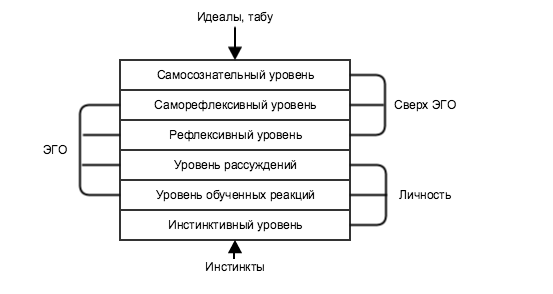
\includegraphics [scale=1.0] {thinkinglevels}
  \caption{Иллюстрация концепции Уровней мышления} 
  \label{img:thinkinglevels}  
\end{figure}
\clearpage
\subsubsection{Концепция k-line}
Концепция K-line была первый раз упомянута Марвином Мински в 1987 году в журнале Cognitive Science. В книге "The Society of Mind" \cite{SocietyOfMind} Марвин Мински раскрывает концепцию K-line. Полностью концепция описана позже в книге "The Emotion Machine" \cite{EmotionMachine}. 
K-line представляет собой связь между двумя событиями, объединяющими их в знание. Например, объединение Пути мышления, найденного решения и активированной проблемы. Данная линия объединяет то как мы думали, решение.
\begin{figure} [h] 
  \center
  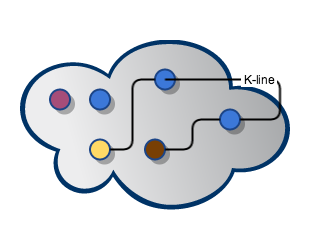
\includegraphics [scale=1.0] {k_line}
  \caption{Иллюстрация концепции K-line} 
  \label{img:k_line}  
\end{figure}
На Рисунке \ref{img:k_line} показана K-line, которая объединяет пути мышления, решение и другие Критики. Данная концепция позволяет "запоминать" удачные решения. 
\clearpage

\section{Выводы}
Модель Menta 0.1 имеет следующие недостатки: отсутствие устойчивости к ошибкам входной информации: грамматическим и содержательным. Например, входной файл не имел отношения к программной системе, модель которой была в базе знаний в формате OWL; система поиска решения работала только в рамках модели одной программы; отсутствовала функция обучения. \par
В данный момент существует новый подход, который использует леса деревьев принятия решений \cite{DCFOREST}, он в рамках данной модели не рассматривался.
Модель Menta 0.3 имеет следующие недостатки: отсутсвие обучения; отсутсвие обработки естественного языка; HyperGraphDB оказалась непригодный для промышленного использования; NARS в виду своих особенностей оказался непригодным для промышленного применения на значительном объеме фактов (>20). Так как содержал в себе комбинаторный взрыв. Например при 10 фактов количество сочетаний будет равно 45 на первом уровне, далее будут сравнивать результаты этих сочетаний; апробации оказалось, что критерии приемки практически описывают необходимое решение, что являлось недопустимым. Данный подход был описан в статье \cite{SECR}. \par

Для программной экспертной системы очень важно обладать способностью мыслить и рассуждать. Например, очень важно  для системы уметь действовать по аналогии. Так как множество запросов типичны и отличаются лишь параметрами. Например, пожалуйста, установить Office, Antivirus и т.д. \par
Также для экспертной системы важно уметь абстрагировать специализированные рецепты решения. К примеру, система научилась решать инцидент "Please install Firefox". Абстрагировав данный инцидент до степени "Please install browser" система сможет теми же способами попробовать решить новый инцидент.\par
После рассмотрения нескольких моделей была выбрана модель мышления Марвина Мински, так как данная модель наиболее точно ложится на целевую область решения инцидентов в области IT. На основе подхода Мински была построена модель системы, которая поддерживает основные функции: обучение, понимание инцидента, поиск решения, применение решения. 

\clearpage

           % Глава 2
\chapter{Вёрстка таблиц} \label{chapt3}

\section{Таблица обыкновенная} \label{sect3_1}

Так размещается таблица:

\begin{table} [htbp]
  \centering
  \parbox{15cm}{\caption{Название таблицы}\label{Ts0Sib}}
%  \begin{center}
  \begin{tabular}{| p{3cm} || p{3cm} | p{3cm} | p{4cm}l |}
  \hline
  \hline
  Месяц   & \centering $T_{min}$, К & \centering $T_{max}$, К &\centering  $(T_{max} - T_{min})$, К & \\
  \hline
  Декабрь &\centering  253.575   &\centering  257.778    &\centering      4.203  &   \\
  Январь  &\centering  262.431   &\centering  263.214    &\centering      0.783  &   \\
  Февраль &\centering  261.184   &\centering  260.381    &\centering     $-$0.803  &   \\
  \hline
  \hline
  \end{tabular}
%  \end{center}
\end{table}

%\newpage
%============================================================================================================================

\section{Параграф - два} \label{sect3_2}

Некоторый текст.

%\newpage
%============================================================================================================================

\section{Параграф с подпараграфами} \label{sect3_3}

\subsection{Подпараграф - один} \label{subsect3_3_1}

Некоторый текст.

\subsection{Подпараграф - два} \label{subsect3_3_2}

Некоторый текст.

\clearpage           % Глава 3
\chapter{ТЕОРЕТИЧЕСКОЕ ОБОСНОВАНИЕ СИСТЕМЫ, АРХИТЕКТУРА И РЕАЛИЗАЦИЯ}
\section{Модель мышления Марвина Мински}
\subsection{Крити-Селектор-Путь мышления}
В 2006 году Марвин Мински опубликовал свою книгу "The emotion machine" \cite{EmotionMachine}, в которой предложил свой взгляд на систему мышления и памяти человека. В основу теории легла парадигма триплета Критик-Селектор-Путь мышления, k-line для сопоставления знаний. На рисунке \ref{img:csw} представлена схематичное изображение Критика-Селектора-Пути мышления \\
\begin{figure} [h] 
  \center
  \includegraphics [scale=1.0] {CSW}
  \caption{Критик-Селектор-Путь мышления} 
  \label{img:csw}  
\end{figure}

\textbf{Критик} представляет собой определенный триггер: внешние обстоятельства, события или иное воздействие. Например, включился свет и зрачки сузились. Обожглись и одернули руку. Критик активируется только когда для этого достаточно обстоятельств. Одновременно могут активироваться несколько критиков. Например, человек решает сложную задачу. Идет активация множество критиков: считать, технические детали, кроме того параллельно может активироваться критик переработки, сообщающей о необходимости отдыха.\\
\textbf{Селектор} занимается выбором определенных ресурсов, которыми также являются Пути мышления. \\
\textbf{Путь мышления} это способ решения проблемы. Путь мышления также может активировать следующий критик. \\

На рисунке \ref{img:csw_ex} представления расширенная модель работы триплета Критик-Селектор-Путь мышления. Критик активирует селектор, который активирует путь мышления (синий круг). Путь мышления в свою очередь может активировать критик или же совершить определенные действия. Например, зажегся зеленый свет светофора, значит можно переходить дорогу. \\
Если активировалось много критиков, значит проблему нужно уточнить, так как степень неопределенности слишком высока. Если проблема очень похожа, то можно судить по аналогии.
\begin{figure} [h] 
  \center
  \includegraphics [scale=1.0] {CSW_EX}
  \caption{Критик-Селектор-Путь мышления в разрезе ресурсов} 
  \label{img:csw_ex}  
\end{figure}

\subsection{Уровни мышления}
Концепция уровней мышления представляет собой степень ментальной активности человека. Никто из людей не может похвастаться скоростью гепарда, гибкости кошки, силой медведя. Но наш вид все это компенсирует возможностью изобретения путей мышления. Например, чтобы быть быстрыми мы изобрели самолеты, машины. Чтобы быть сильными, мы изобрели оружие. Что же делает это возможным? Безусловно результатом всего является взаимодействие человека с окружающим миром. Именно данное взаимодействие заставляет людей изобретать что-то новое, создавать шедевры литературы и летать в космос. Но как же мы всего этого добиваемся начиная от, инстинктивного одергивая руки до создания Теории всего \cite{Hawking}. Далее мы рассмотрим концепцию уровней мышления.
\begin{enumerate}
	\item Инстинктивный уровень
	\item Уровень обученных реакций
	\item Уровень рассуждений
	\item Рефлексивный уровень
	\item Саморефлексивный уровень
	\item Самосознательный уровень
\end{enumerate}
\textbf{Инстинктивный уровень.} На данном уровне происходят инстинктивные реакции (врожденные). Например, боязнь обжечься. Не прыгать под машину. Общую формулу для этого уровня можно выразить как "Если ..., то сделать так".\\
\textbf{Уровень обученных реакций.} На  данной уровне происходит мышление обученных реакций, то есть тех реакций, которыми человек обучается в течение жизни. Например, переходить дорогу на зеленых свет. Общую формулу для этого уровня можно выразить как "Если ..., то сделать так". \\
\textbf{Уровень рассуждений.} На  данной уровне происходит мышление с использованием рассуждений. Если я сделаю так, то будет ... Например, если перебежать дорогу на зеленый свет, то можно успеть вовремя. На данном уровне сравниваются последствия нескольких решений и выбирается оптимальное. Общую формулу для этого уровня можно выразить как "Если ..., то сделать так, тогда будет так". \\
\textbf{Рефлексивный уровень.} На данном уровне происходит рассуждение с учетом анализа прошлых событий. Например, прошлый раз я побежал на моргающий зеленый и чуть не попал под машину.\\
\textbf{Саморефлексивный уровень.} На данном уровне происходит оценка себя. Строится определенная модель с помощью которой идет оценка своих поступков. Например, мое решение не пойти на это собрание было неверным, так как я упустил столько возможностей, я был \textbf{легкомысленный}.\\
\textbf{Самосознательный уровень.} Самозонательный уровень на данный момент характерен только для человека. На данном уровне идет оценка поступков человека с точки зрения высших идеалов и внешних оценок. Например, а что подумают мои друзья? А как бы поступил мой герой? \\
Деление на данные уровне носит условный характер. Например уровень 5 и 6 можно объединить. Но по словам Марвина Мински принцип бритвы Оккама успешно применяется в физики, но в психологии он не должен применяться также легко. \\
На рисунке \ref{img:thinkinglevels} представлена схематичное изображение уровней мышления. 1-3 уровни составляют личность человека. 2-5 представляют ЭГО человека (Человеческое Я) - осознание человека в общении с окружающими. 3-6 представляют собой сверх ЭГО человека (сверх Я) - его моральные установки.
\begin{figure} [h] 
  \center
  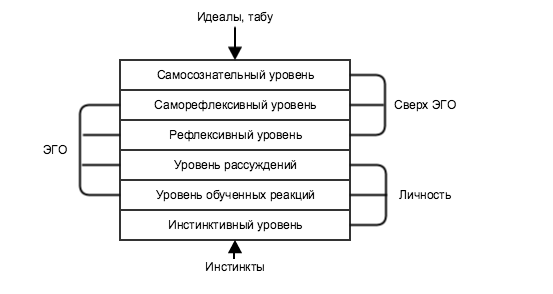
\includegraphics [scale=1.0] {thinkinglevels}
  \caption{Критик-Селектор-Путь мышления в разрезе ресурсов} 
  \label{img:thinkinglevels}  
\end{figure}

%\newpage
%============================================================================================================================




\clearpage           % Глава 4
\chapter*{ЗАКЛЮЧЕНИЕ}						% Заголовок
\addcontentsline{toc}{chapter}{ЗАКЛЮЧЕНИЕ}	% Добавляем его в оглавление

%% Согласно ГОСТ Р 7.0.11-2011:
%% 5.3.3 В заключении диссертации излагают итоги выполненного исследования, рекомендации, перспективы дальнейшей разработки темы.
%% 9.2.3 В заключении автореферата диссертации излагают итоги данного исследования, рекомендации и перспективы дальнейшей разработки темы.
%% Поэтому имеет смысл сделать эту часть общей и загрузить из одного файла в автореферат и в диссертацию:

%% Согласно ГОСТ Р 7.0.11-2011:
%% 5.3.3 В заключении диссертации излагают итоги выполненного исследования, рекомендации, перспективы дальнейшей разработки темы.
%% 9.2.3 В заключении автореферата диссертации излагают итоги данного исследования, рекомендации и перспективы дальнейшей разработки темы.

Решены следующие задачи и достигнуты следующие результаты.
\begin{enumerate}
  \item Создана модель проблемно-ориентированной системы управления, принятия решений в области обслуживания информационной структуры предприятия на основе модели мышления;
  \item Представлены новая модель данных для модели мышления и оригинальный способ ее хранения, эффективный по сравнению с другими базами данных;
  \item Выполнено оригинальное исследование моделей мышления в области обслуживания информационной структуры предприятия;
  \item На основе модели созданы архитектура системы и ее прототип; 
  \item Созданы специальные алгоритмы для анализа запросов пользователей и принятия решений;
  \item Система, разработанная в рамках данной работы, включает в себя инновационные методы и алгоритмы поддержки принятия решений, использует модель мышления на базе модели мышления Мински;
  \item Представлена наглядная визуализация структуры области удаленной поддержки инфраструктуры.
\end{enumerate}

Представленные в диссертации модель мышления, ее архитектура и реализация являются уникальными~--- на данный момент времени это единственная реализация модели мышления Мински. \par
Система, разработанная в диссертации, не является узкоспециализированной. Она также подходит для других областей, где требуется поддержка принятия решений. Например, при постановке медицинского диагноза, чтобы отбросить ложные диагнозы. \par
Кроме того, в систему можно загрузить данные о взаимосвязи органов человека и болезней. Далее, к каждому заболеванию добавить симптом и способ лечения, после этого можно делать запрос с симптомами, и система выдаст список вероятных заболеваний со способами их лечения. \par
В области диагностики проблем можно обучить систему узлам автомобиля, проблемам, с ними связанными, признаками этих проблем и способами их устранения. 





Работа велась с использованием открытых технологий, без использования проприетарного программного обеспечения. Работа была презентована автору книги Object-Oriented Software Construction \cite{Meyer} Бертрану Мейеру в рамках серии лекций, проведенных при содействии Университета Иннополис в Казани в 2015 году в рамках AKSES-2015 http://university.innopolis.ru/en/research/selab/events/akses и была им отмечена.  
Работа выполнялась при помощи компании ОАО "АйСиЭл КПО ВС", в рамках работы использовались и обрабатывались данные, собранные во время работы команд ICL над поддержкой информационной структуры предприятий-заказчиков.      % Заключение
\chapter*{Список сокращений и условных обозначений}             % Заголовок
\addcontentsline{toc}{chapter}{Список сокращений и условных обозначений}  % Добавляем его в оглавление

\textbf{selectLinkedObject(obj:Resource, linkName:String): Link<Resource>}~--- Описание метода. selectLinkedObject~--- название метода. (obj:Resource, linkName:String)~--- параметры метода. linkName~--- имя параметра. String тип данных. Link<Resource>~--- тип возвращаемых данных. Если метод данных не возвращает, то ничего не указывается.\\

\textbf{TU}~--- Сокращение от ThinkingUnderstanding.\\

\textbf{TLC}~--- Thinking Life Cycle.\\

\textbf{НДФЛ}~--- Налог на доходы физически лиц.\\

\textbf{ПО}~--- Программное обеспечение.\\

\clearpage
      % Список сокращений и условных обозначений
\chapter*{Словарь терминов}             % Заголовок
\addcontentsline{toc}{chapter}{Словарь терминов}  % Добавляем его в оглавление

\textbf{База Знаний}~--- База данных приложения, представленная в виде онтологии знаний. \\

\textbf{WayToThink}~--- Путь мышления. Основан на определении Марвина Мински \cite{EmotionMachine}. Класс объектов, которые модифицируют данные. \\

\textbf{Critic}~--- Основан на определении Марвина Мински \cite{EmotionMachine}. Класс объектов, которые выступают триггерами при наступление определенного события. \\

\textbf{ThinkingLifeCycle}~--- Основан на определении Марвина Мински \cite{EmotionMachine}. Класс объектов, которые выступают основными объектами для запуска в приложении~--- рабочими процессами. \\

\textbf{Selector}~--- Компонент, отвечающий за выборку данных из Базы Знаний. \\

\textbf{Instinctive}~--- Инстинктивный уровень. \\

\textbf{Learned}~--- Уровень обученных реакций. \\

\textbf{Deliberative}~--- Уровень рассуждений. \\

\textbf{Reflective}~--- Рефлексивный уровень. \\

\textbf{Self-Reflective Thinking	}~--- Саморефлексивный уровень. \\

\textbf{Self-Conscious Reflection}~--- Самосознательный уровень. \\

\textbf{ThinkingUnderstanding}~--- Система, созданная в рамках работы. Дословный перевод "Мышление-Понимание".\\  

\textbf{Вариант использования}~--- Термин из стандарта UML, который описывает возможные способы функционирования системы.\\  

\textbf{Диаграмма действий}~--- Термин из стандарта UML, который описывает последовательность действий пользователя.\\   
 
\clearpage    % Словарь терминов
\clearpage
\phantomsection
\addcontentsline{toc}{chapter}{\bibname}	% Добавляем список литературы в оглавление
\bibliography{biblio}						% Подключаем BibTeX-базы      % Список литературы
\clearpage
\phantomsection
\addcontentsline{toc}{chapter}{\listfigurename}
\listoffigures									% Список изображений
\newpage

%%% Список таблиц %%%
% (ГОСТ Р 7.0.11-2011, 5.3.10)
\clearpage
\phantomsection
\addcontentsline{toc}{chapter}{\listtablename}
\listoftables									% Список таблиц
\newpage           % Списки таблиц и изображений (иллюстративный материал)
\appendix
\chapter{Приложение А. Интерфейсная модель} \label{AppendixA}

Интерфейсная модель содержит классы и интерфейсы для взаимодействия с пользователем.

\begin{figure} [h] 
  \center
  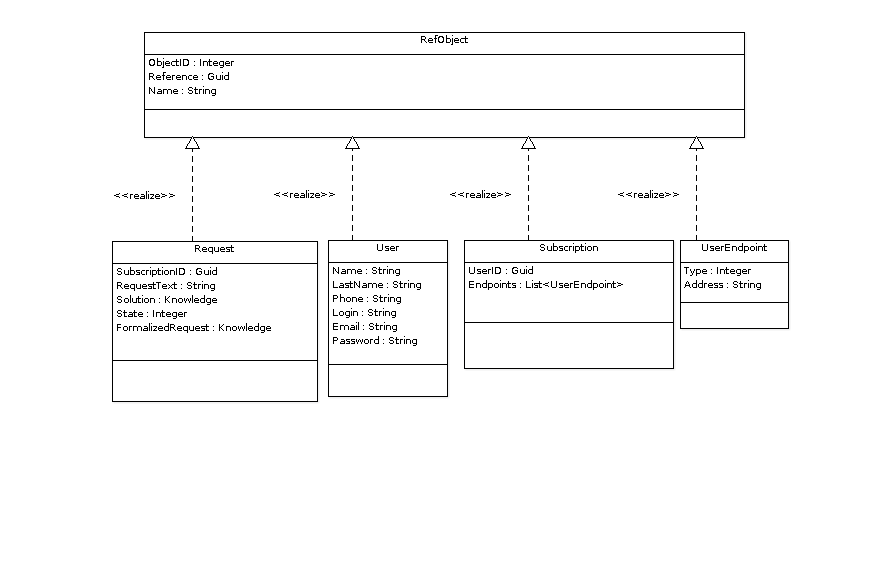
\includegraphics [scale=0.8,angle=90, origin=c] {interface-model}
  \caption{Диаграмма классов интерфейсной модели} 
  \label{img:interface-model}  
\end{figure}

\emph{RefObject}

Представляет собой общий объект, который сохраняется в Базе Знаний. (Базовый класс для всех остальных классов и объектов)
\begin{itemize}
	\item ObjectID- уникальный в пределах класса ключ
	\item Reference- уникальный в пределах всех баз знаний ключ
	\item Name-имя объекта
\end{itemize}

\emph{Request}

Объект для хранения запроса пользователя.
\begin{itemize}
	\item SubscriptionID - идентификатор подписки
	\item RequestText - запрос пользователя в виде текста
	\item Solution - ссылка на решение запроса
	\item State - статус запроса (например, Поиск Решения)
	\item FormalizedRequest - ссылка на формализованный запрос
\end{itemize}


\emph{Subscription}

Информация о подписке пользователя на события
\begin{itemize}
	\item Endpoints - списко UserEndpoint, которые будут использоваться для обратной связи с пользователем
\end{itemize}

\emph{UserEndpoint}
\begin{itemize}
	\item Type - тип точки связи с пользователем (например, веб-сервис)
	\item Address - адрес точки связи с пользователем
\end{itemize}

\chapter{Приложение B. Action} \label{AppendixB}
Action является базовым классом для WayToThink или Critic.
\begin{figure} [h] 
  \center
  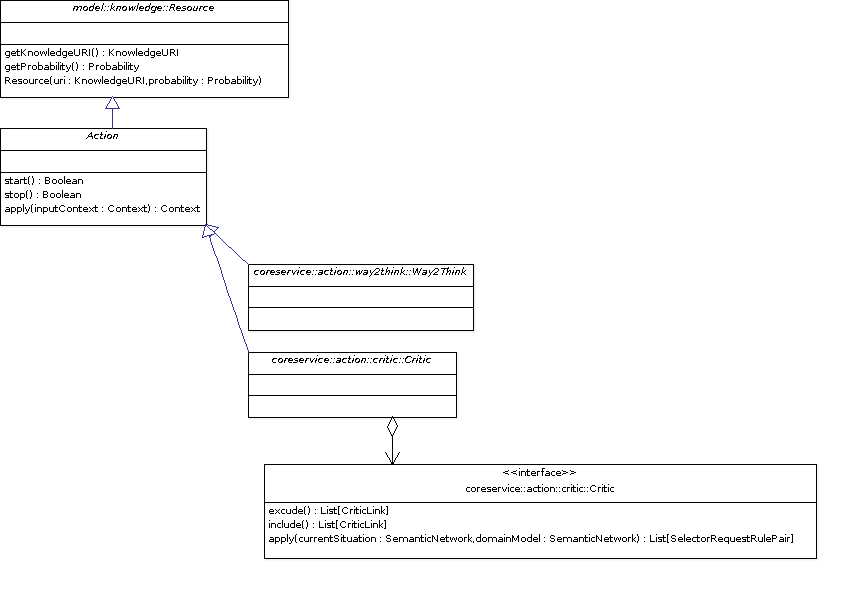
\includegraphics [scale=0.6, origin=c] {ActionClass}
  \caption{Диаграмма классов Action} 
  \label{img:ActionClass}  
\end{figure}



\chapter{Очень длинное название второго приложения, в котором продемонстрирована работа с длинными таблицами} \label{AppendixBX}

 \section{Подраздел приложения}\label{AppendixB1}
Вот размещается длинная таблица:
\fontsize{10pt}{10pt}\selectfont
\begin{longtable}[c]{|l|c|l|l|}
% \caption{Описание входных файлов модели}\label{Namelists} 
%\\ 
 \hline
 %\multicolumn{4}{|c|}{\textbf{Файл puma\_namelist}}        \\ \hline
 Параметр & Умолч. & Тип & Описание               \\ \hline
                                              \endfirsthead   \hline
 \multicolumn{4}{|c|}{\small\slshape (продолжение)}        \\ \hline
 Параметр & Умолч. & Тип & Описание               \\ \hline
                                              \endhead        \hline
 \multicolumn{4}{|r|}{\small\slshape продолжение следует}  \\ \hline
                                              \endfoot        \hline
                                              \endlastfoot
 \multicolumn{4}{|l|}{\&INP}        \\ \hline 
 kick & 1 & int & 0: инициализация без шума ($p_s = const$) \\
      &   &     & 1: генерация белого шума                  \\
      &   &     & 2: генерация белого шума симметрично относительно \\
  & & & экватора    \\
 mars & 0 & int & 1: инициализация модели для планеты Марс     \\
 kick & 1 & int & 0: инициализация без шума ($p_s = const$) \\
      &   &     & 1: генерация белого шума                  \\
      &   &     & 2: генерация белого шума симметрично относительно \\
  & & & экватора    \\
 mars & 0 & int & 1: инициализация модели для планеты Марс     \\
kick & 1 & int & 0: инициализация без шума ($p_s = const$) \\
      &   &     & 1: генерация белого шума                  \\
      &   &     & 2: генерация белого шума симметрично относительно \\
  & & & экватора    \\
 mars & 0 & int & 1: инициализация модели для планеты Марс     \\
kick & 1 & int & 0: инициализация без шума ($p_s = const$) \\
      &   &     & 1: генерация белого шума                  \\
      &   &     & 2: генерация белого шума симметрично относительно \\
  & & & экватора    \\
 mars & 0 & int & 1: инициализация модели для планеты Марс     \\
kick & 1 & int & 0: инициализация без шума ($p_s = const$) \\
      &   &     & 1: генерация белого шума                  \\
      &   &     & 2: генерация белого шума симметрично относительно \\
  & & & экватора    \\
 mars & 0 & int & 1: инициализация модели для планеты Марс     \\
kick & 1 & int & 0: инициализация без шума ($p_s = const$) \\
      &   &     & 1: генерация белого шума                  \\
      &   &     & 2: генерация белого шума симметрично относительно \\
  & & & экватора    \\
 mars & 0 & int & 1: инициализация модели для планеты Марс     \\
kick & 1 & int & 0: инициализация без шума ($p_s = const$) \\
      &   &     & 1: генерация белого шума                  \\
      &   &     & 2: генерация белого шума симметрично относительно \\
  & & & экватора    \\
 mars & 0 & int & 1: инициализация модели для планеты Марс     \\
kick & 1 & int & 0: инициализация без шума ($p_s = const$) \\
      &   &     & 1: генерация белого шума                  \\
      &   &     & 2: генерация белого шума симметрично относительно \\
  & & & экватора    \\
 mars & 0 & int & 1: инициализация модели для планеты Марс     \\
kick & 1 & int & 0: инициализация без шума ($p_s = const$) \\
      &   &     & 1: генерация белого шума                  \\
      &   &     & 2: генерация белого шума симметрично относительно \\
  & & & экватора    \\
 mars & 0 & int & 1: инициализация модели для планеты Марс     \\
kick & 1 & int & 0: инициализация без шума ($p_s = const$) \\
      &   &     & 1: генерация белого шума                  \\
      &   &     & 2: генерация белого шума симметрично относительно \\
  & & & экватора    \\
 mars & 0 & int & 1: инициализация модели для планеты Марс     \\
kick & 1 & int & 0: инициализация без шума ($p_s = const$) \\
      &   &     & 1: генерация белого шума                  \\
      &   &     & 2: генерация белого шума симметрично относительно \\
  & & & экватора    \\
 mars & 0 & int & 1: инициализация модели для планеты Марс     \\
kick & 1 & int & 0: инициализация без шума ($p_s = const$) \\
      &   &     & 1: генерация белого шума                  \\
      &   &     & 2: генерация белого шума симметрично относительно \\
  & & & экватора    \\
 mars & 0 & int & 1: инициализация модели для планеты Марс     \\
kick & 1 & int & 0: инициализация без шума ($p_s = const$) \\
      &   &     & 1: генерация белого шума                  \\
      &   &     & 2: генерация белого шума симметрично относительно \\
  & & & экватора    \\
 mars & 0 & int & 1: инициализация модели для планеты Марс     \\
kick & 1 & int & 0: инициализация без шума ($p_s = const$) \\
      &   &     & 1: генерация белого шума                  \\
      &   &     & 2: генерация белого шума симметрично относительно \\
  & & & экватора    \\
 mars & 0 & int & 1: инициализация модели для планеты Марс     \\
kick & 1 & int & 0: инициализация без шума ($p_s = const$) \\
      &   &     & 1: генерация белого шума                  \\
      &   &     & 2: генерация белого шума симметрично относительно \\
  & & & экватора    \\
 mars & 0 & int & 1: инициализация модели для планеты Марс     \\
 \hline
  %& & & $\:$ \\ 
 \multicolumn{4}{|l|}{\&SURFPAR}        \\ \hline
kick & 1 & int & 0: инициализация без шума ($p_s = const$) \\
      &   &     & 1: генерация белого шума                  \\
      &   &     & 2: генерация белого шума симметрично относительно \\
  & & & экватора    \\
 mars & 0 & int & 1: инициализация модели для планеты Марс     \\
kick & 1 & int & 0: инициализация без шума ($p_s = const$) \\
      &   &     & 1: генерация белого шума                  \\
      &   &     & 2: генерация белого шума симметрично относительно \\
  & & & экватора    \\
 mars & 0 & int & 1: инициализация модели для планеты Марс     \\
kick & 1 & int & 0: инициализация без шума ($p_s = const$) \\
      &   &     & 1: генерация белого шума                  \\
      &   &     & 2: генерация белого шума симметрично относительно \\
  & & & экватора    \\
 mars & 0 & int & 1: инициализация модели для планеты Марс     \\
kick & 1 & int & 0: инициализация без шума ($p_s = const$) \\
      &   &     & 1: генерация белого шума                  \\
      &   &     & 2: генерация белого шума симметрично относительно \\
  & & & экватора    \\
 mars & 0 & int & 1: инициализация модели для планеты Марс     \\
kick & 1 & int & 0: инициализация без шума ($p_s = const$) \\
      &   &     & 1: генерация белого шума                  \\
      &   &     & 2: генерация белого шума симметрично относительно \\
  & & & экватора    \\
 mars & 0 & int & 1: инициализация модели для планеты Марс     \\
kick & 1 & int & 0: инициализация без шума ($p_s = const$) \\
      &   &     & 1: генерация белого шума                  \\
      &   &     & 2: генерация белого шума симметрично относительно \\
  & & & экватора    \\
 mars & 0 & int & 1: инициализация модели для планеты Марс     \\
kick & 1 & int & 0: инициализация без шума ($p_s = const$) \\
      &   &     & 1: генерация белого шума                  \\
      &   &     & 2: генерация белого шума симметрично относительно \\
  & & & экватора    \\
 mars & 0 & int & 1: инициализация модели для планеты Марс     \\
kick & 1 & int & 0: инициализация без шума ($p_s = const$) \\
      &   &     & 1: генерация белого шума                  \\
      &   &     & 2: генерация белого шума симметрично относительно \\
  & & & экватора    \\
 mars & 0 & int & 1: инициализация модели для планеты Марс     \\
kick & 1 & int & 0: инициализация без шума ($p_s = const$) \\
      &   &     & 1: генерация белого шума                  \\
      &   &     & 2: генерация белого шума симметрично относительно \\
  & & & экватора    \\
 mars & 0 & int & 1: инициализация модели для планеты Марс     \\ 
 \hline 
\end{longtable}

\fontsize{14pt}{15pt}\selectfont
\section{Ещё один подраздел приложения} \label{AppendixB2}

Нужно больше подразделов приложения!

\section{Очередной подраздел приложения} \label{AppendixB3}

Нужно больше подразделов приложения!

\section{И ещё один подраздел приложения} \label{AppendixB4}

Нужно больше подразделов приложения!

        % Приложения

\end{document}
